\documentclass[11pt,a4paper]{article}
\usepackage[utf8]{inputenc}
\usepackage{amsmath}
\usepackage{mathptm}
\usepackage{amsfonts}
\usepackage{amssymb}
\usepackage{graphicx}
\usepackage[a4paper]{geometry}
\usepackage[hyphens]{url}
\geometry{top=35mm, left=30mm, right=30mm, bottom=35mm}
\renewcommand{\contentsname}{Inhaltsverzeichnis}
\usepackage{graphicx}
\usepackage{float}

\begin{document}
\begin{titlepage}
\begin{figure}
\centering
%\includegraphics[scale=5]{pics/2015_10_05_FHB_Logo_RGB_fbw.png}
\end{figure}
\title{Kali Linux Ausarbeitung}
\date{}

\maketitle
\end{titlepage}

\newpage
%\tableofcontents

\section {Installation von Kali Linux auf Android mit Linux Deploy auf Asus}
%\newpage

Die Installation von Kali Linux Distribution auf das  Asus-Gerät befolgt die folgenden Anweisungen:

\subsection{gerootetes Android-Tablet für diese Installation erforderlich}
Das Gerät muss gerootet sein.
"Root" unter Android ist ganz wichtig.
Im Grunde bezeichnet "root" ein Nutzer, der volle Zugriffs- und Schreibrechte auf das System hat. Eine Wurzel oder root-Konto Zugriff wird häufig mit Administratorrechten auf Windows verglichen, obwohl es einige Unterschiede im Detail gibt. Ein Root-Konto oder ein Root-Zugriff wird daher oft mit den Administratorrechten unter Windows verglichen, auch wenn es im Detail einige Unterschiede gibt.

Es gibt viele Vorteile, wenn ein Gerät gerootet ist. Beispiele: \\
- Funktionen nachrüsten (z.B. Multi-User auf Handys) \\
- CPU/GPU-Anpassungen (z.B. für mehr Leistung)  \\


\subsection{Die administrativen Rechte durch SuperSU}
Die administrativen Rechte unter Android werden durch Root-Apps wie \textbf{SuperSU} und \textbf{Superuser} geregelt, das heißt, jede andere App, die Root-Rechte fordert, muss durch eine der eben genannten Apps manuell freigegeben werden. \\

Das folgende Bild zeigt die Schritte zu folgen: \\

\begin{figure}[!h]
\begin{center} 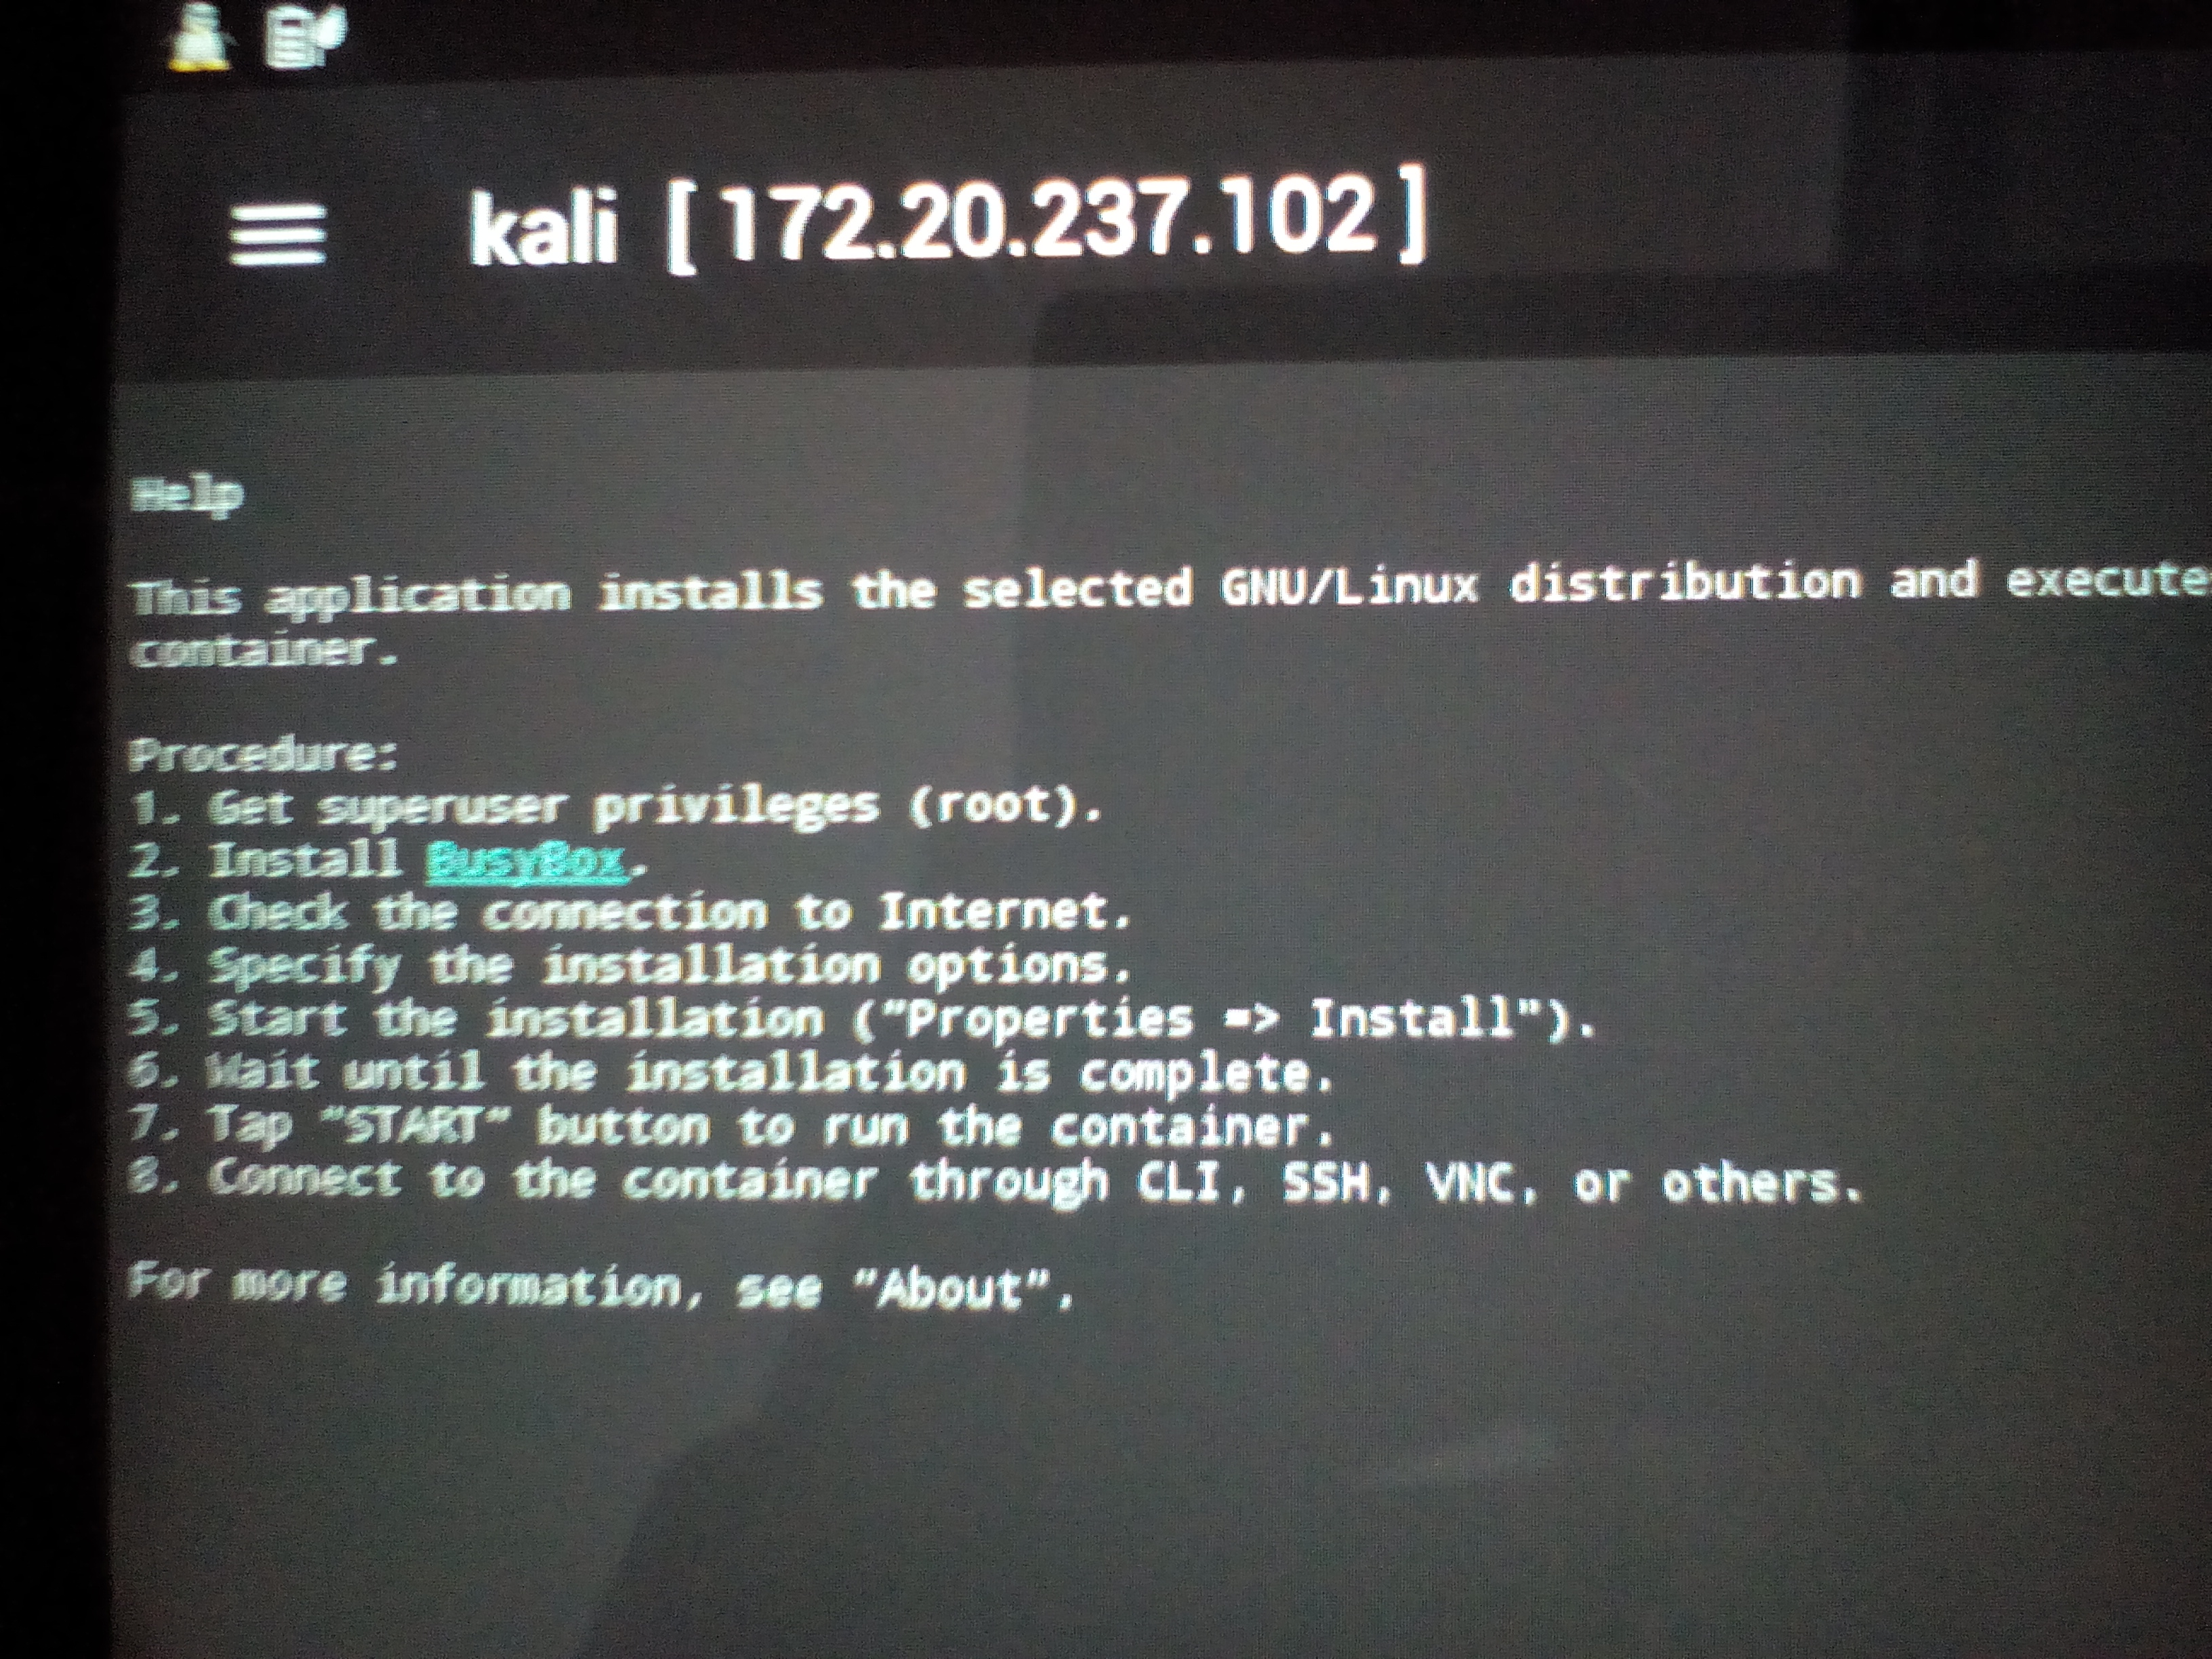
\includegraphics[scale=0.09]{./Image/img1}  \\
\caption{Schritte}
\end{center}
\end{figure}


\subsection{Gute Internet-Verbindung}
Alle benötigten Pakete werden aus unseren Repositories heruntergeladen, das heißt Sie benötigen eine schnelle Internetverbindung, um diese Installationsmethode zu verwenden. \\

\subsection{Mindestens 5GB  Freier Platz}
Lassen Sie mindestens 5GB auf der internen oder externen Speicher frei. 

  
 \subsection{benötigte App}  
 
Die drei folgenden App sind vor der Installation von Kali Linux zu installieren.

 \textbf{Die Virtuelle Maschine Busy Box}  \\ 
 
Busybox ist eine Software, die viele der Standard-Unix-Befehle, wie die GNU Core Utilities implementiert.

Da jede ausführbare Binärdatei für GNU / Linux mehrere Kilobyte zusätzliche Informationen enthält,die Idee von kombinieren  mehr als zweihundert Programme in eine ausführbare Datei ist gut.
BusyBox ist eine freie Software. \\
 
 
\textbf{Linux Deploy} \\

Diese Anwendung ist Open-Source-Software für die schnelle und einfache Installation des Betriebssystems (OS) GNU / Linux auf Ihrem Android-Gerät. \\

Die Anwendung erstellt ein Disk-Image auf einer Flash-Karte, montiert es und installiert eine OS-Verteilung. Anwendungen des neuen Systems werden in einer chroot-Umgebung ausgeführt und arbeiten mit der Android-Plattform zusammen. \\



 \textbf{Android VNC Viewer} \\
 "VNC Viewer" ist ein kostenloser VNC-Client für Android. 
 VNC Viewer" ermöglicht den Fernzugriff auf Linux.

       
Wir müssen auch die Parameter von Kali Linux Überprüfen 
Diese Parameter sind in der Figure 2, 3 und 4 veranschaulicht.\\ 

In der Figure 2 sind die Parameter wie folgt konfiguriert:

- Die Architektur: armhf \\
- Distribution Suite: Kali-Rolling \\
- Quellpfad: http://http.kali.org/kali/ \\
- Installation Pfad: \$\{EXTERNAL\_ STORAGE\}\/linux.img  \\
- Image Größe(MB): Automatische Berechnung \\
- Dateisystem: Auto \\
- Benutzername: Kali \\
- Benutzerpassword: kali0123 \\
- Privileged Users: Root \\
- DNS Server: Automatische Erkennung \\

\begin{figure}[!h]
\begin{center} 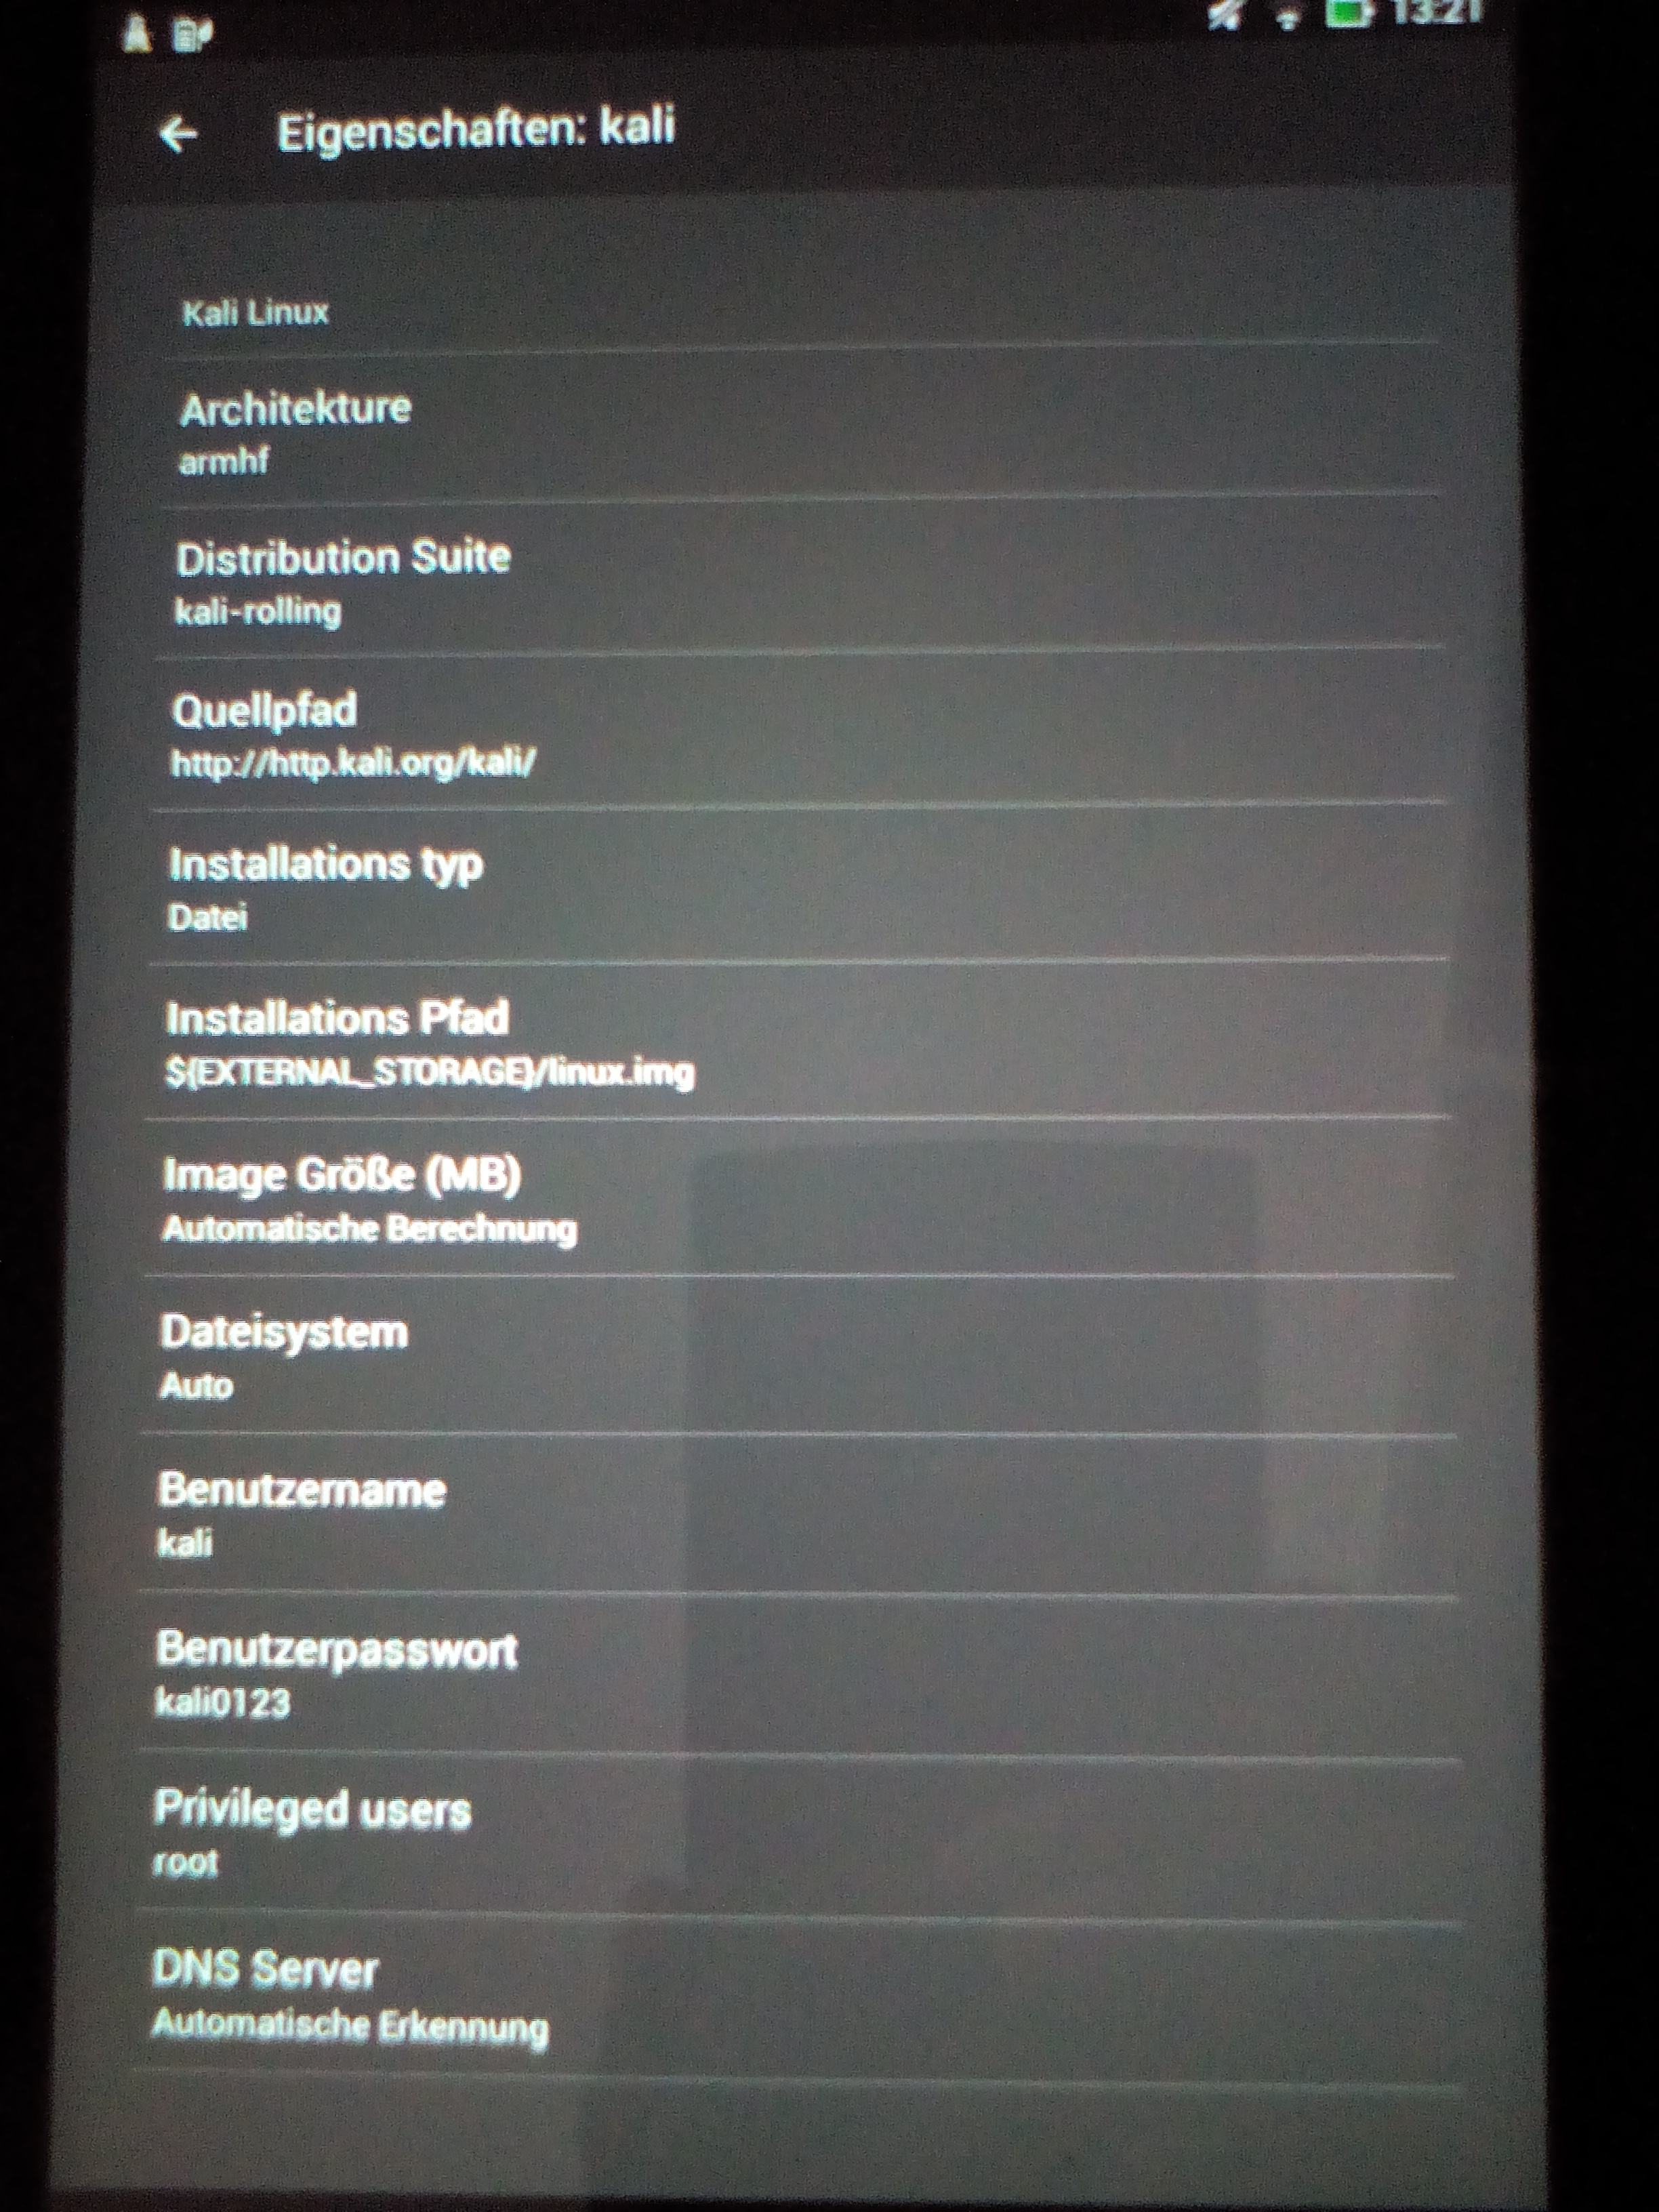
\includegraphics[scale=0.1]{./Image/img2}  \\
\caption{Parameter1}
\end{center}
\end{figure}

In der Figure 3 sind die Parameter wie folgt konfiguriert: \\
-SSH Enable (Erlaube das Mount der Android Resources) \\
-GUI Enable (Die Desktopumgebung wird beim Start des Linux-Systems hochgefahren) \\

\begin{figure}[H]
\begin{center} 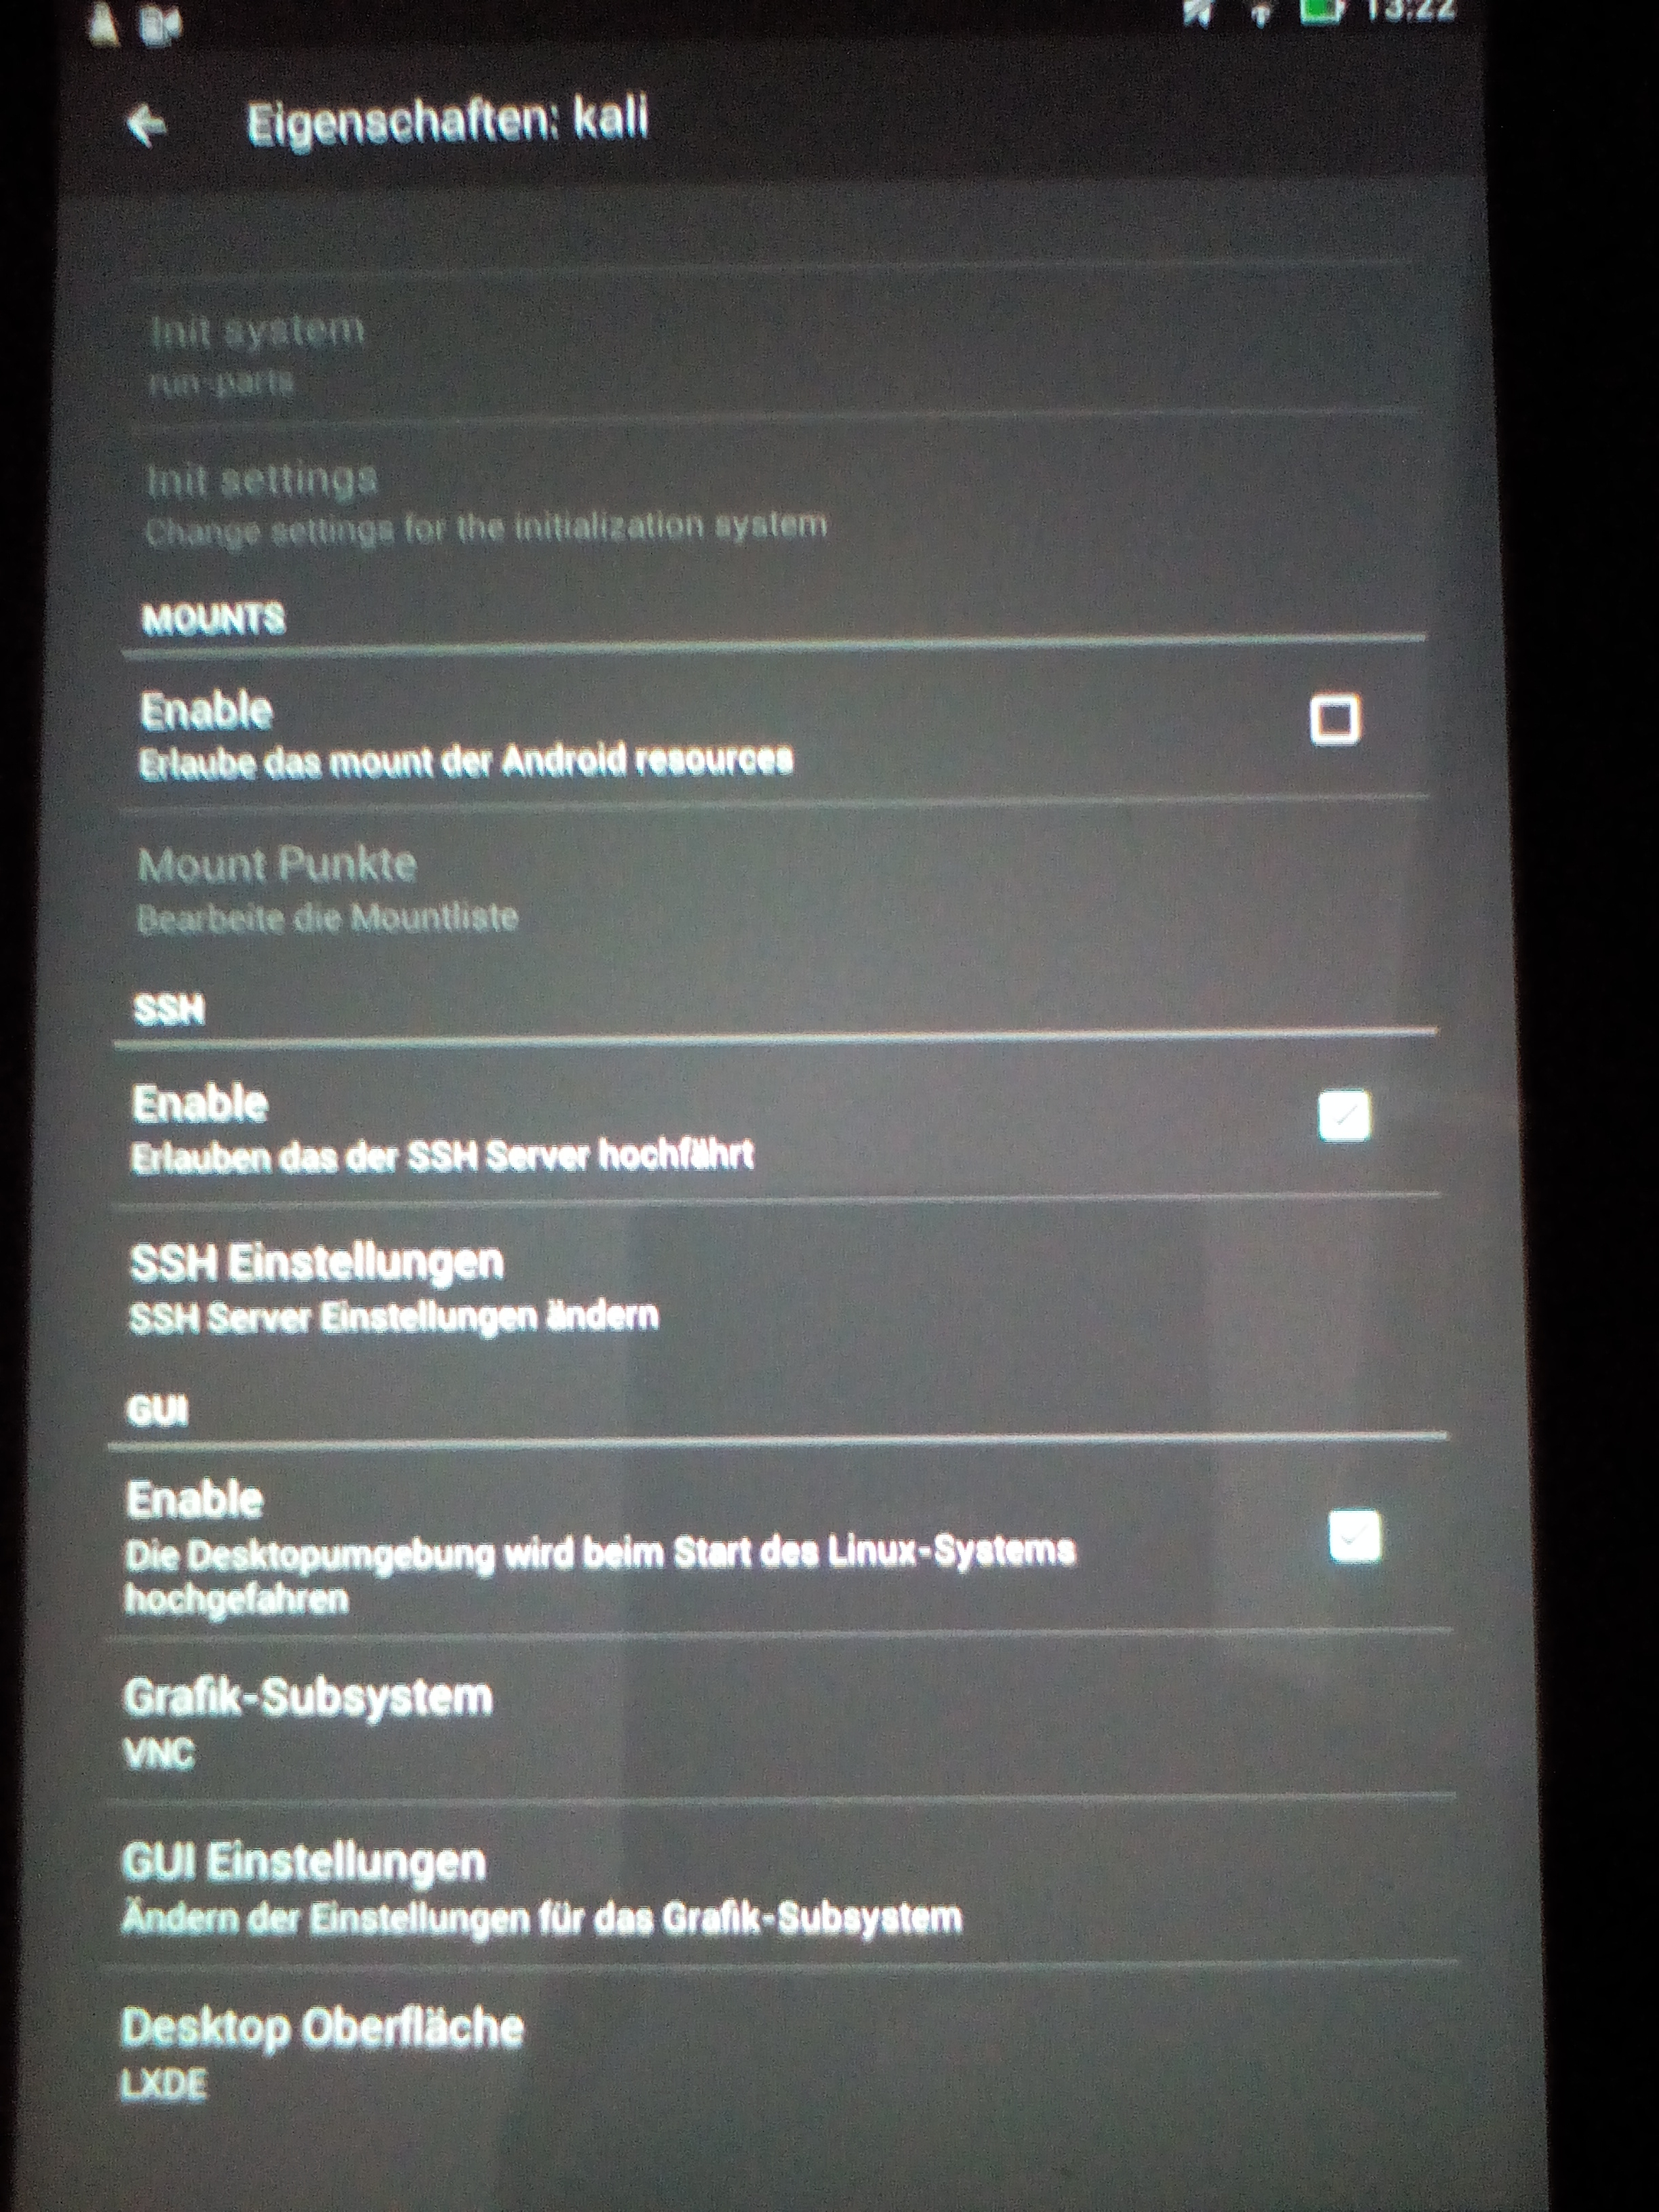
\includegraphics[scale=0.1]{./Image/img3}  \\
\caption{Parameter2}
\end{center}
\end{figure} 

\subsection{install und Konfigure}

- Dann klicken wir auf \textbf{Install} (Properties $\rightarrow$ Install) \\
Sobald die Einstellungen fertig sind, klicken wir auf "Install". Diese Aktion wird einen Kali Linux-Bootstrap direkt aus den Repositories starten. Diese Vorgang nimmt ungefähr 30 Minuten Zeit in Anspruch. Wir laden eine Basisinstallation von Kali Linux auf Minimum herunter. \\ 

- Dann klicken auf \textbf{Configure} \\
Die Figure 4 zeigt wie das aussieht. 

\begin{figure}[H]
\begin{center} 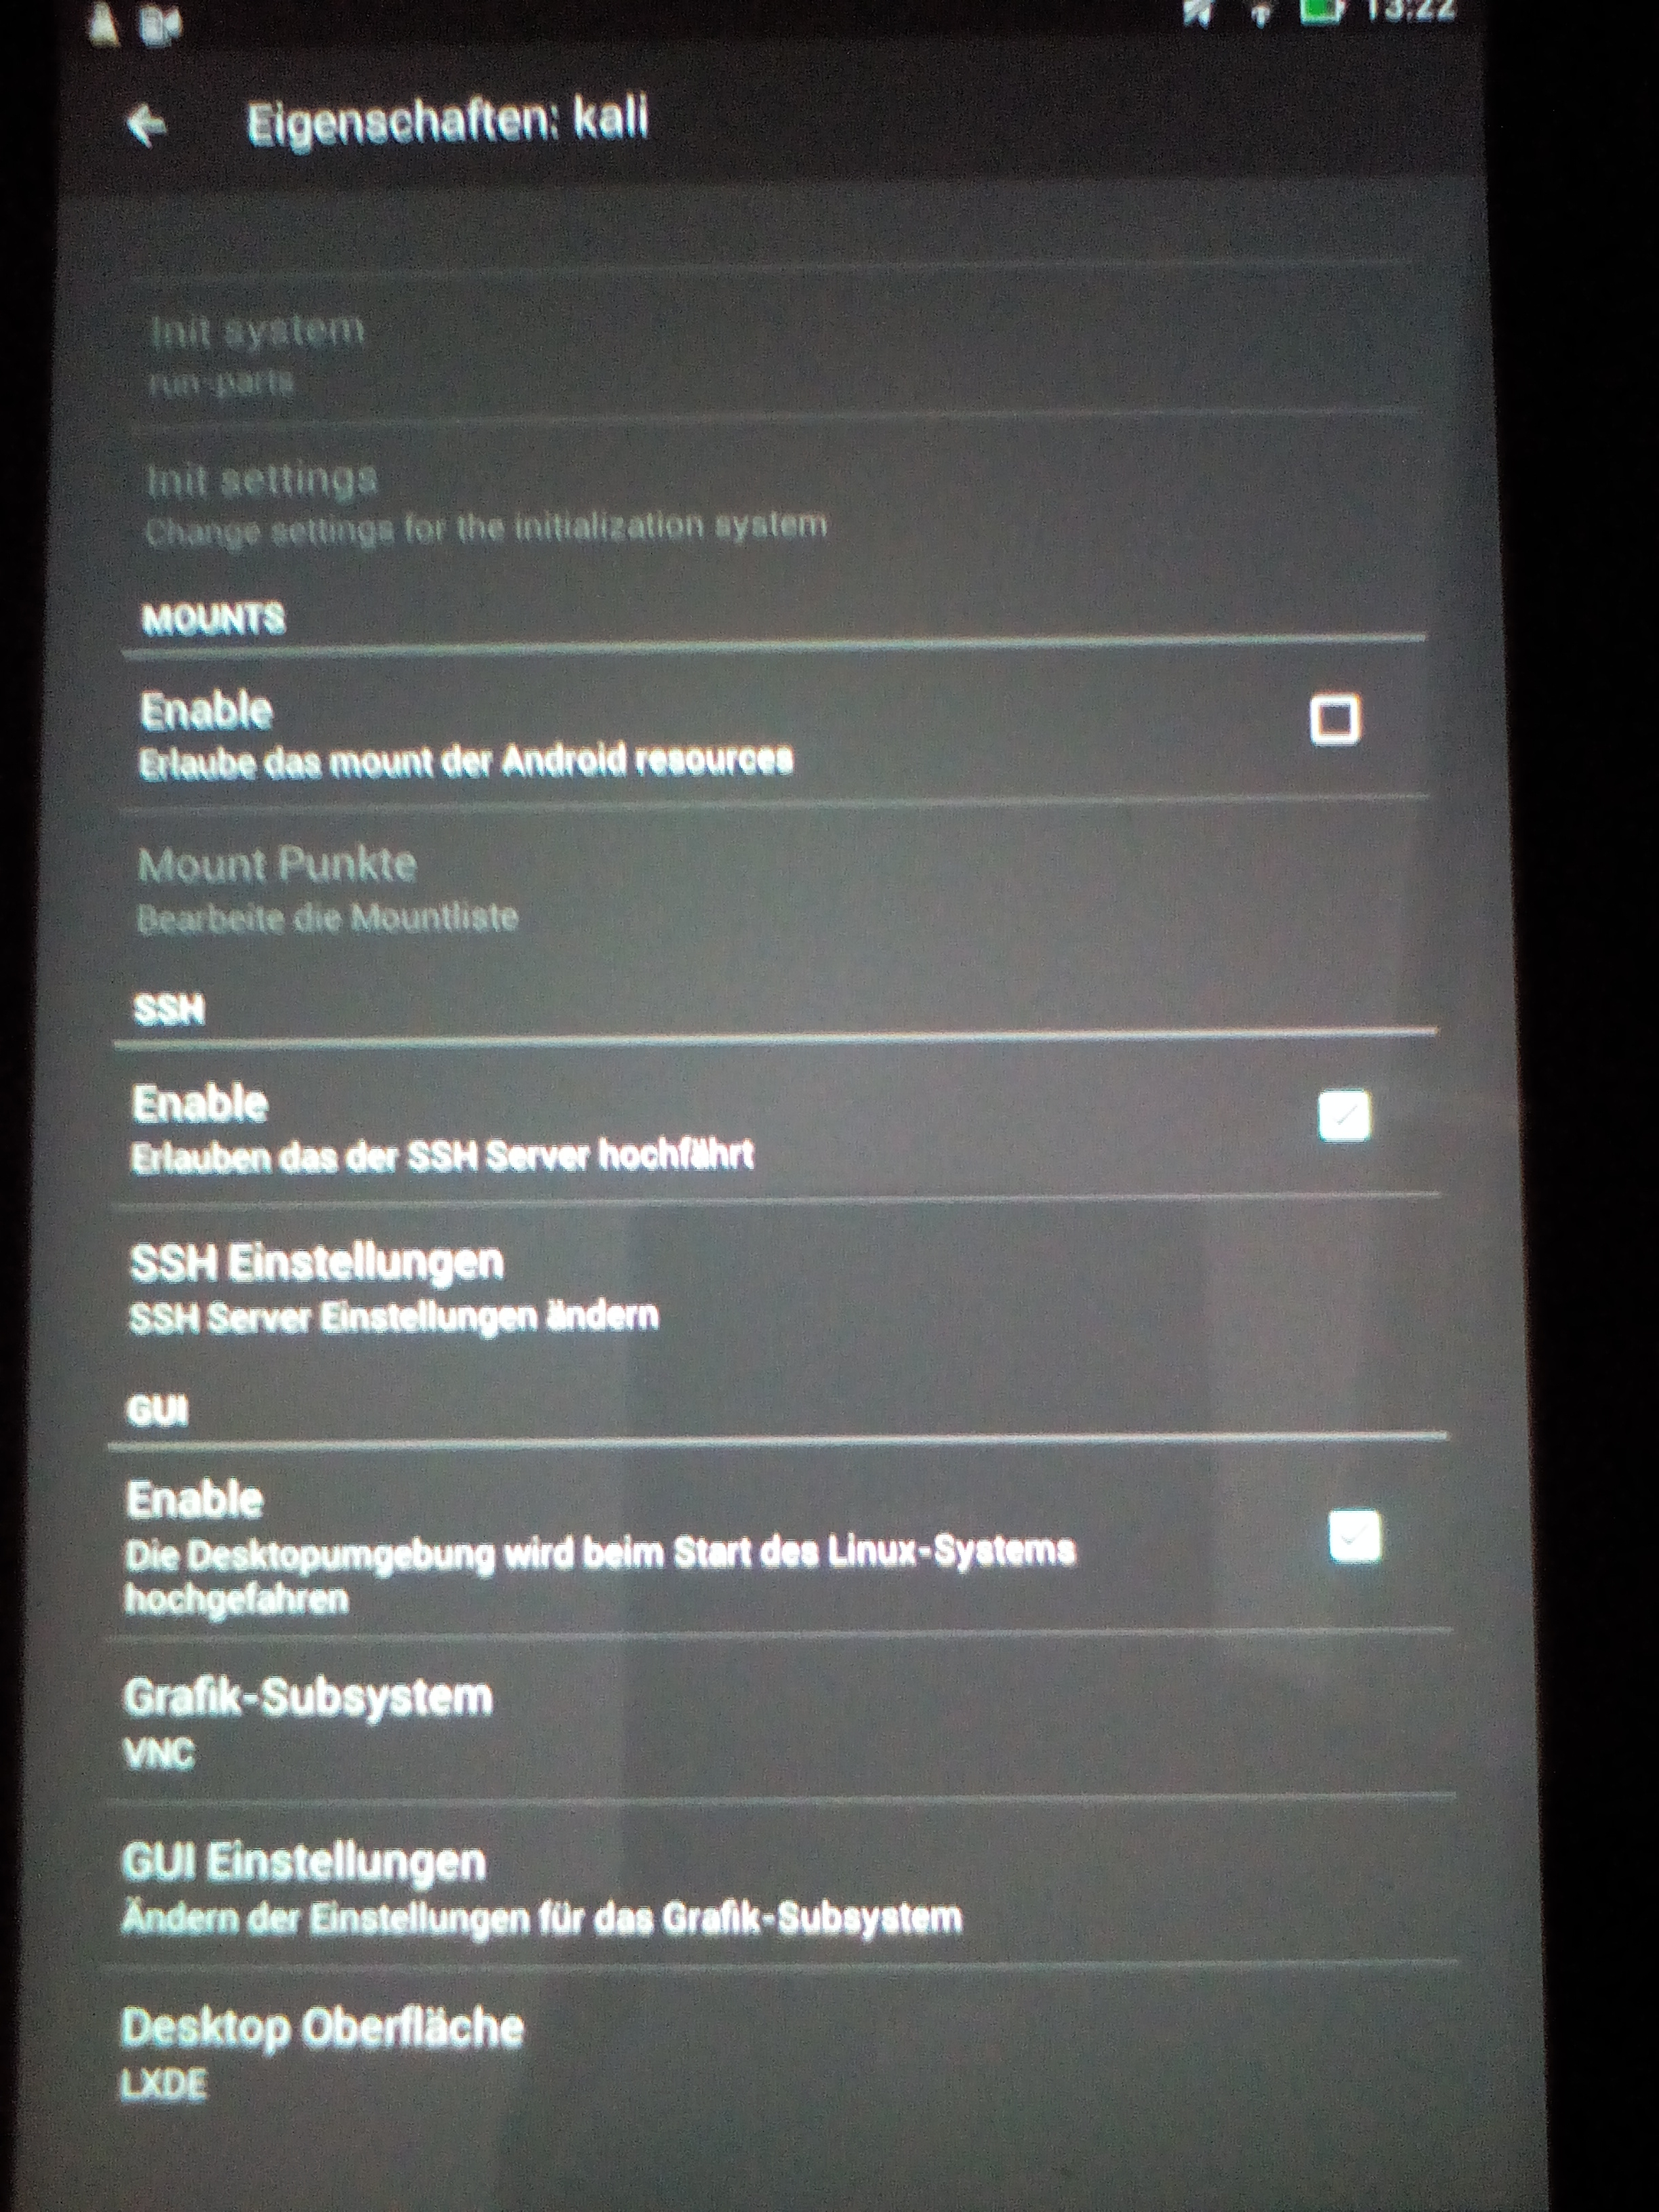
\includegraphics[scale=0.1]{./Image/img4}  \\
\caption{Install und configure}
\end{center}
\end{figure} 

- Dann klicken auf \textbf{Start} \\ \\

\begin{figure}[H]
\begin{center} 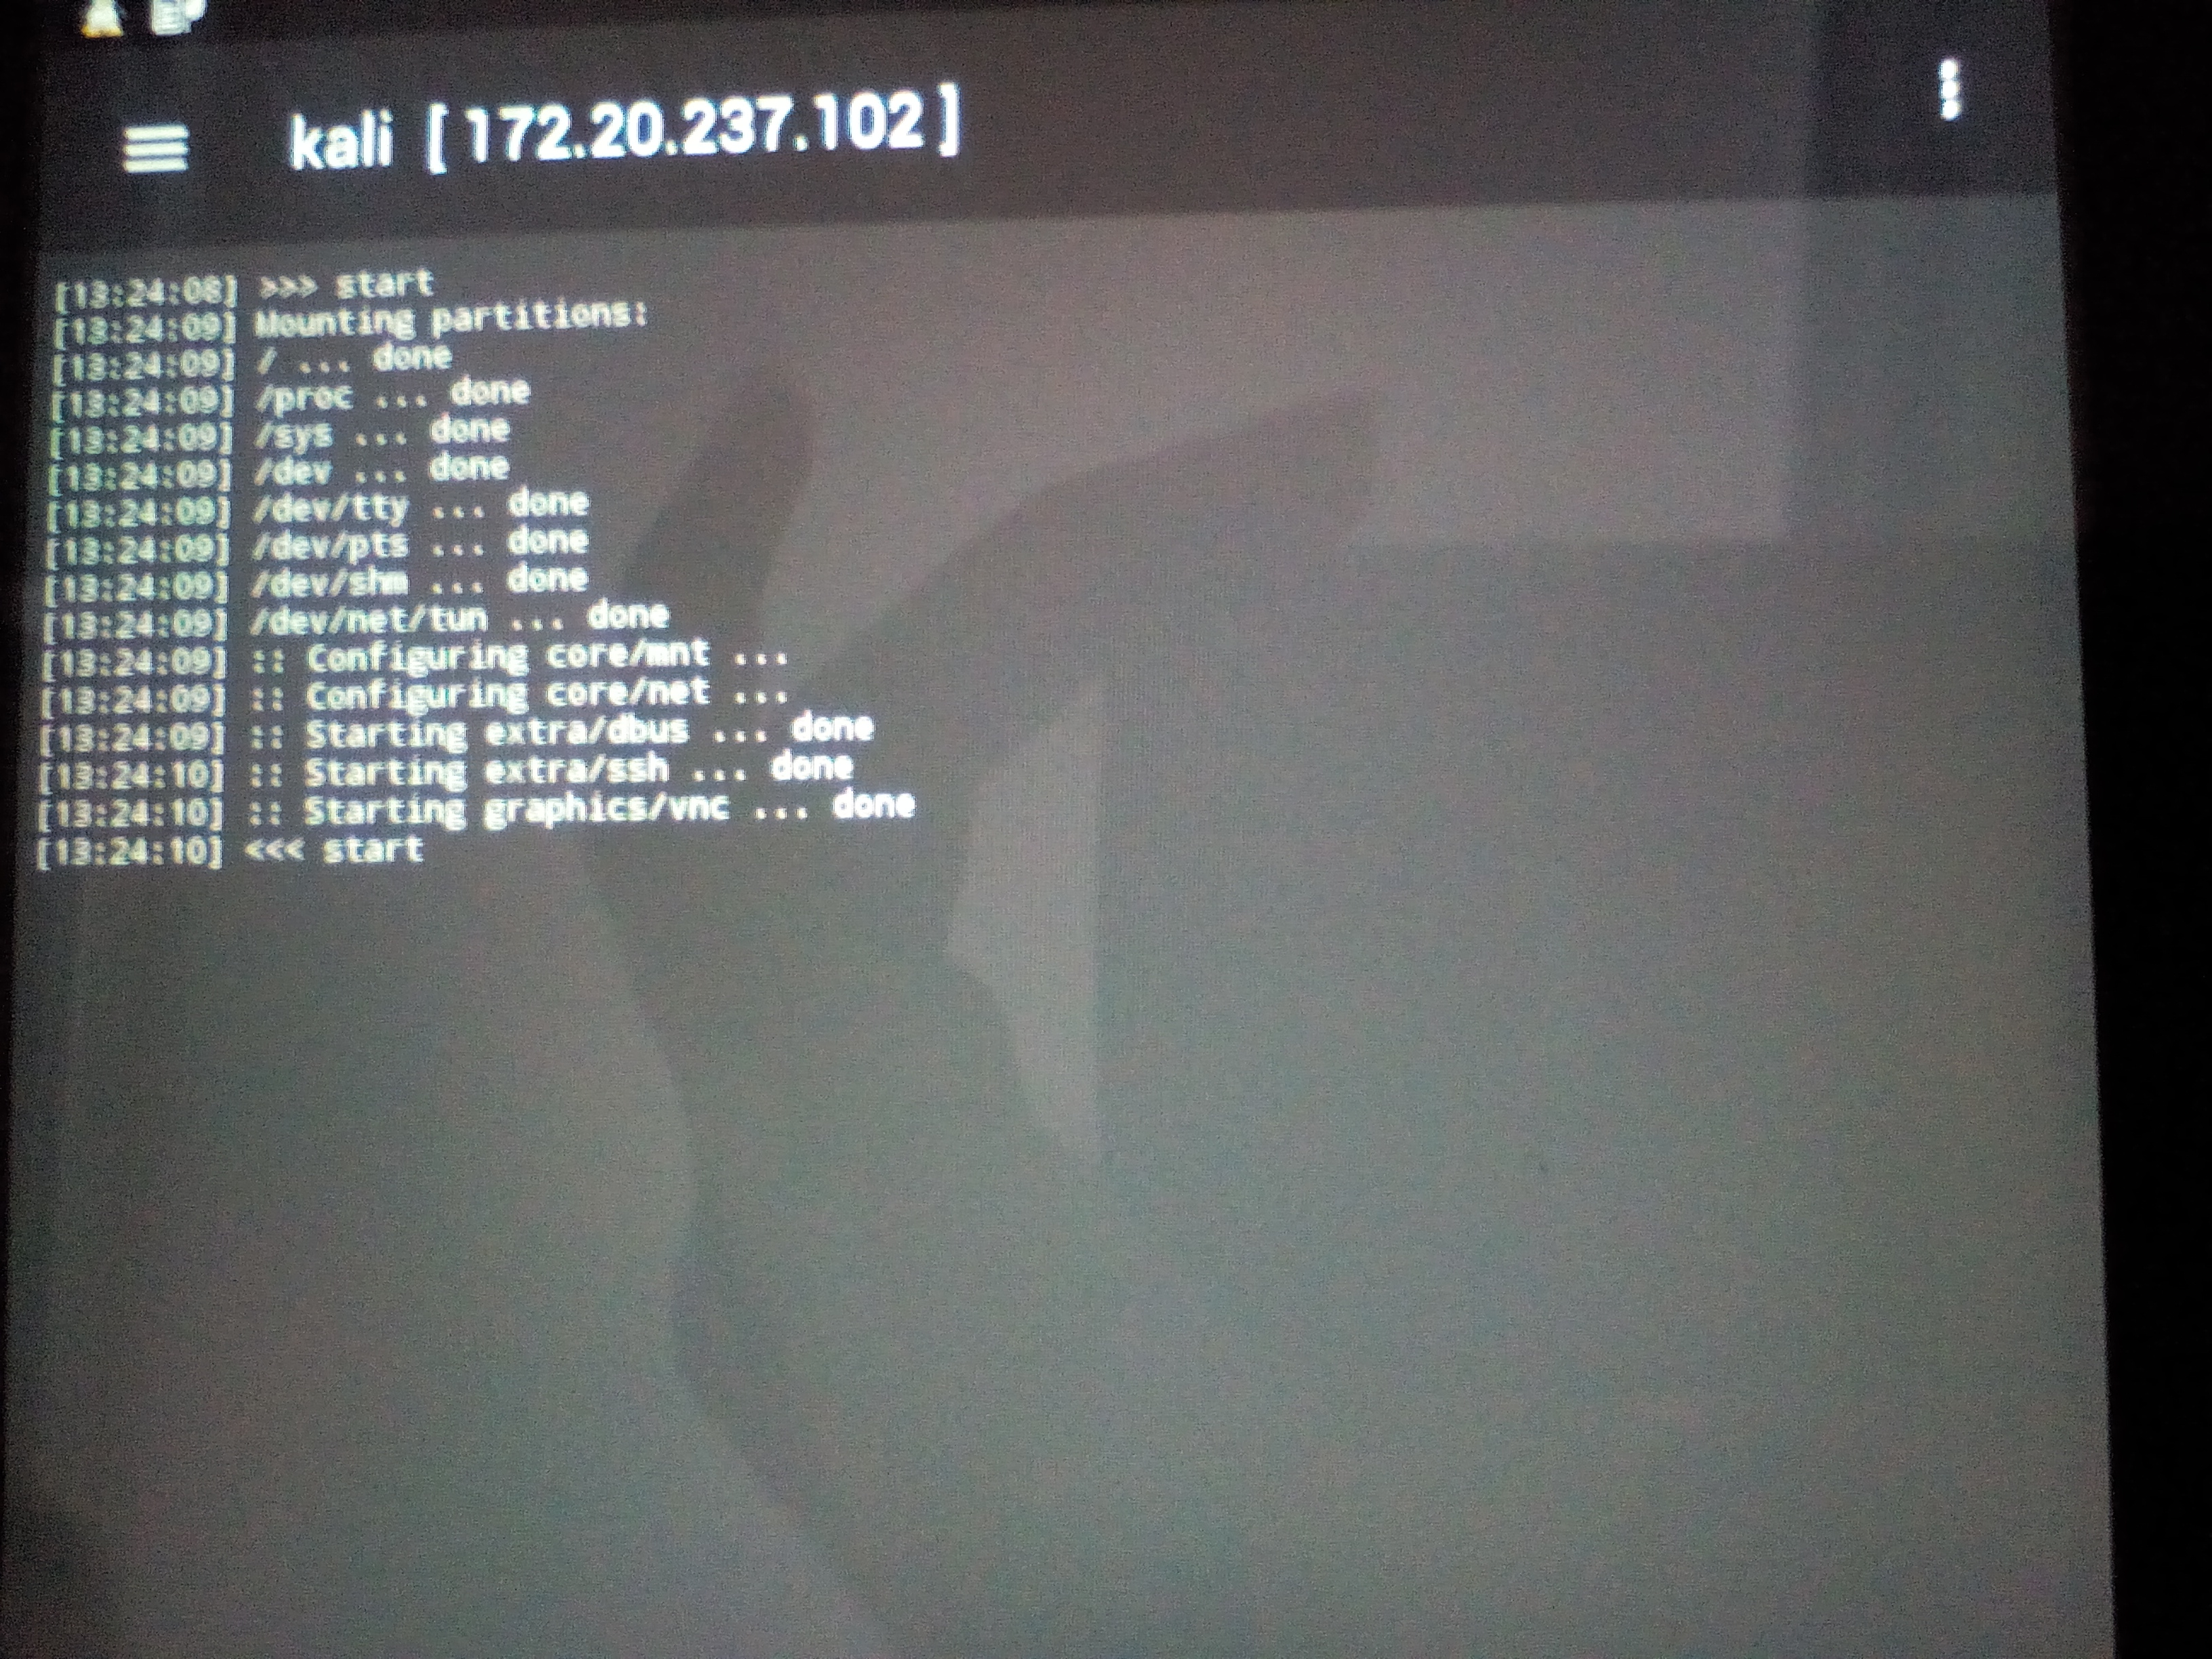
\includegraphics[scale=0.1]{./Image/img5}  \\
\caption{Installation}
\end{center}
\end{figure} 

- Jetzt wir warten auf das Ende der Installation \\
Sobald die Installation abgeschlossen ist, können wir Linux Deploy automatisch installiert und laden das Kali Linux Chroot-Image. Dazu gehört auch der Start von Diensten wie SSH und VNC für leichteren Fernzugriff. All dies geschieht automagisch, indem man den "Start" -Button drückt. 

\subsection{Meldung mit Android VNC Viewer}
Wir melden uns an Android VNC Viewer mit der Super User Parameter \\
Schauen die Figure 6 an. \\

\begin{figure}[H]
\begin{center} 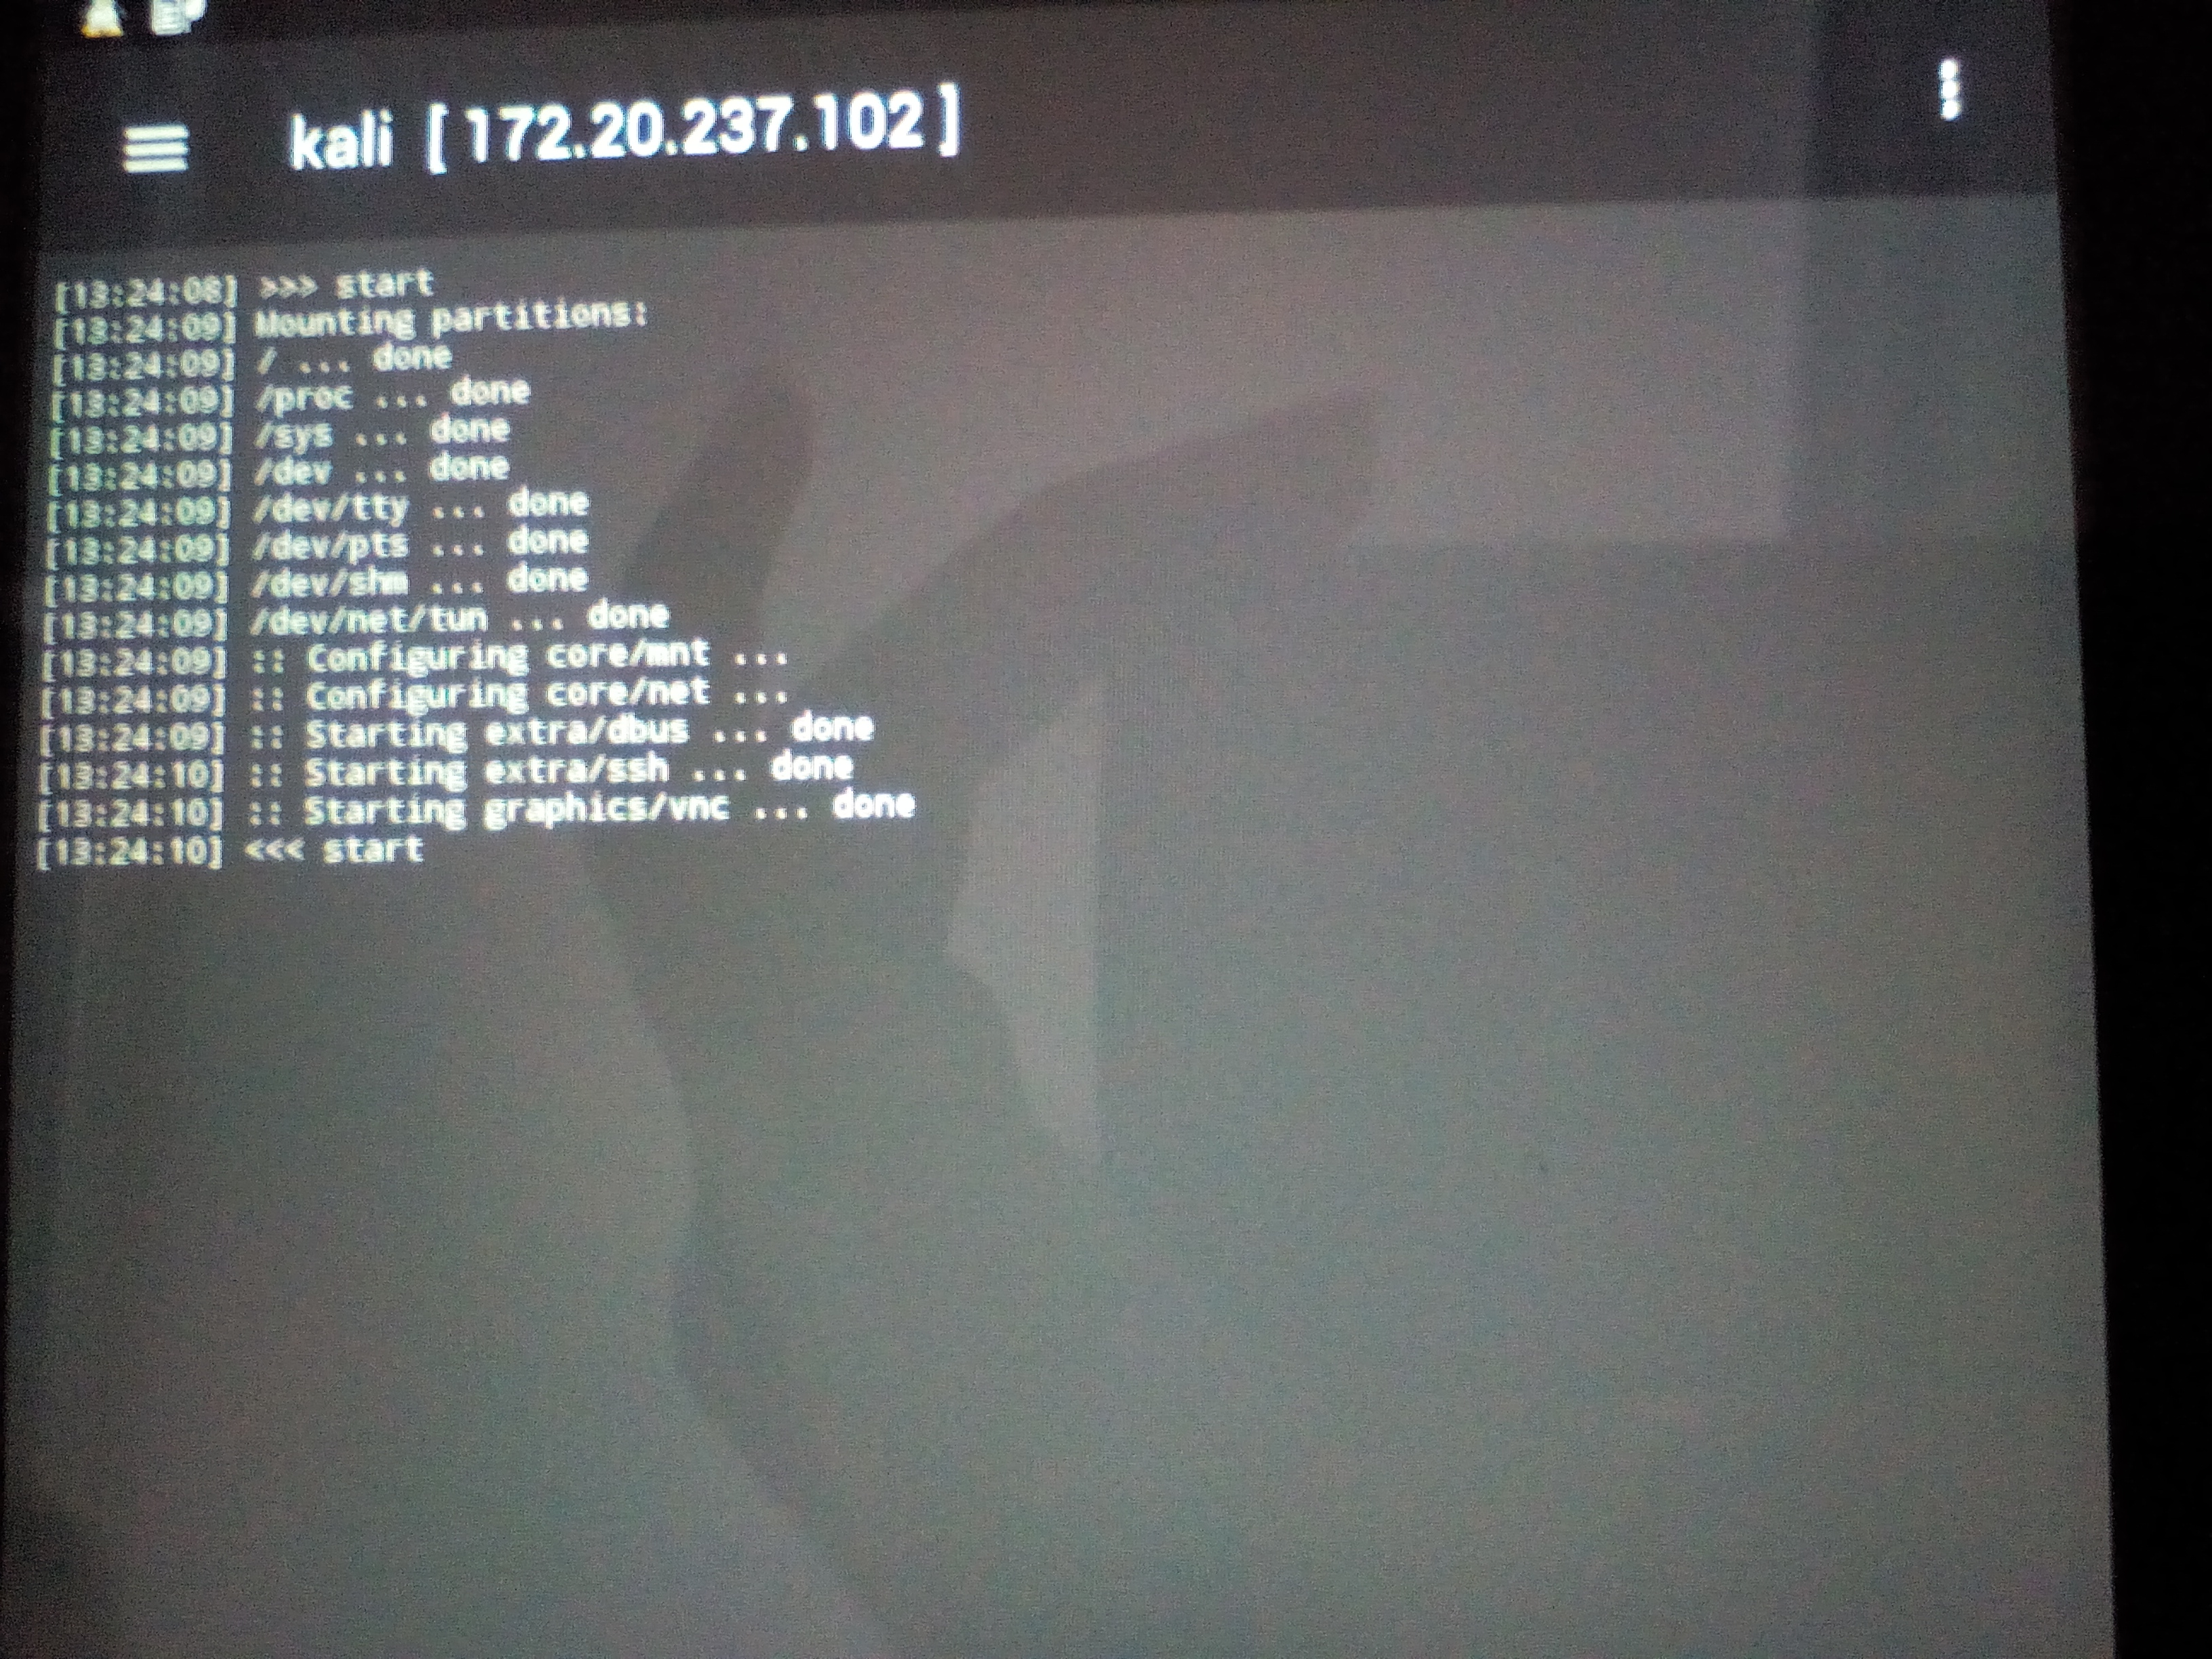
\includegraphics[scale=0.1]{./Image/img6}  \\
\caption{VNC Viewer Anmeldung}
\end{center}
\end{figure} 

Die GUI von VNC Viewer erscheint in Figure 7 \\
\begin{figure}[H]
\begin{center} 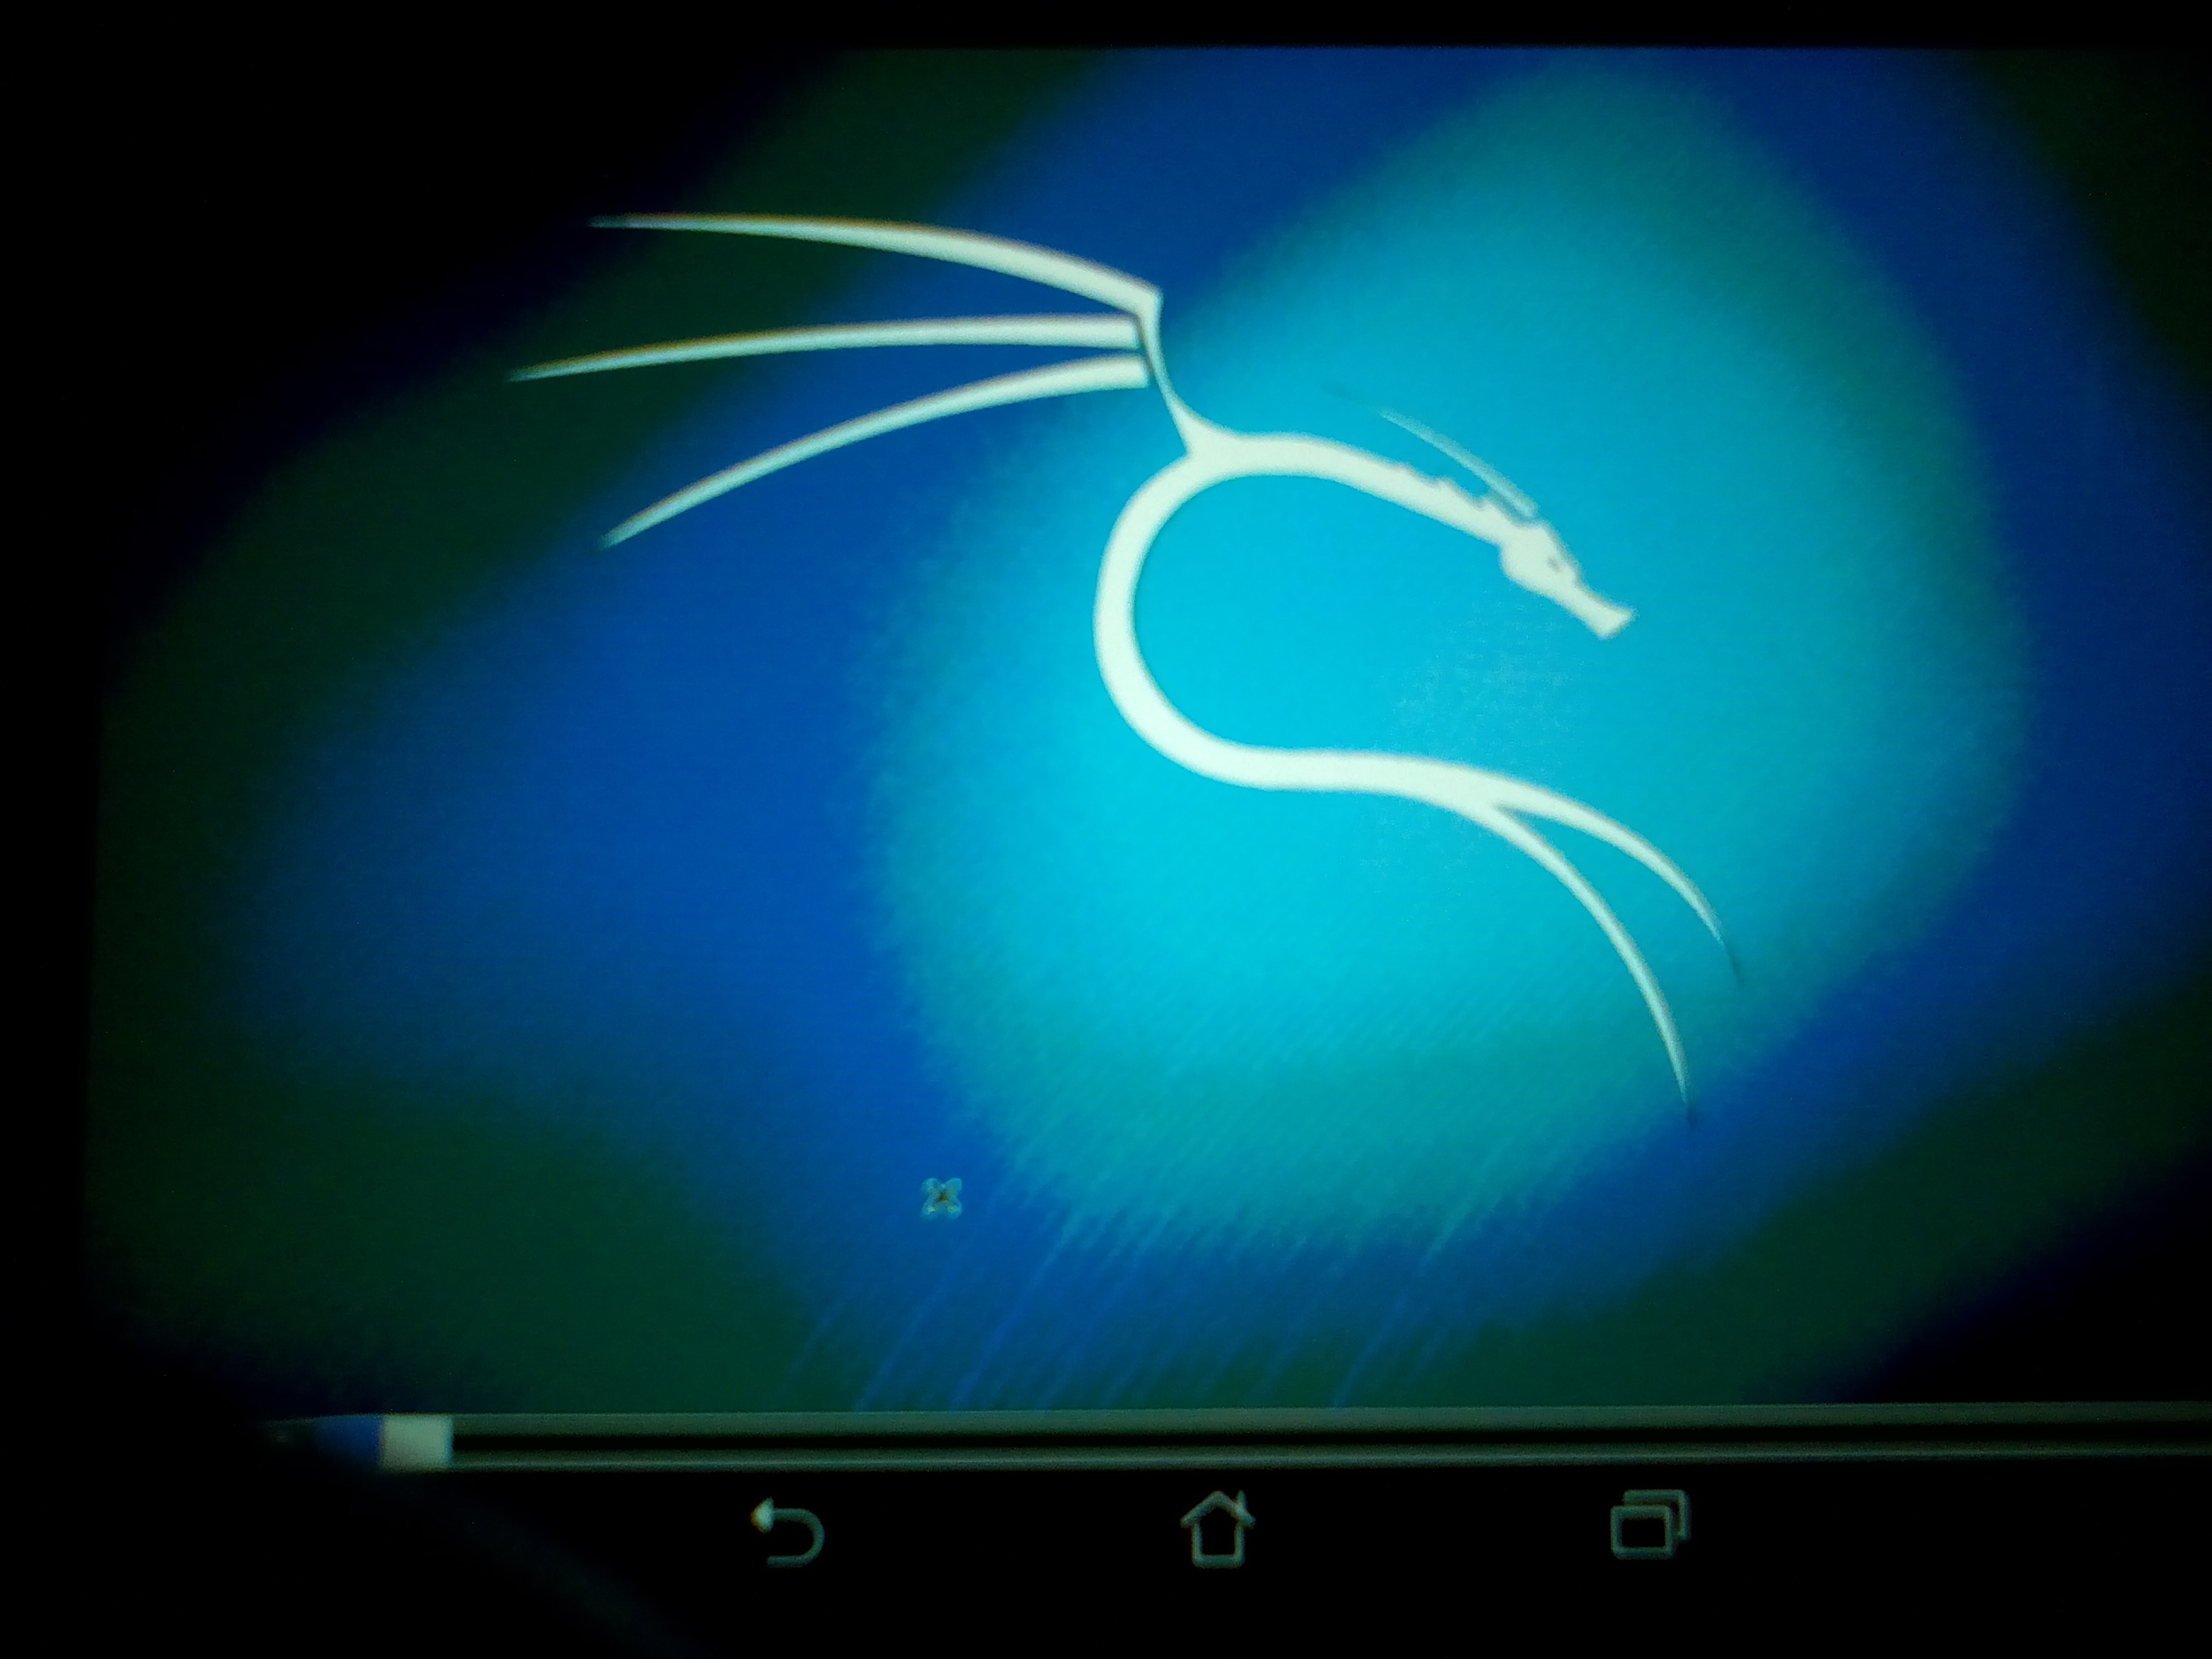
\includegraphics[scale=0.1]{./Image/img7}  \\
\caption{GUI VNC Viewer}
\end{center}
\end{figure} 

Literatur Installing and und Running Kali Linux with Linux Deploy: \footnote{http://www.compsmag.com/install-kali-linux-android/}

\section {Installation von Nethunter auf Nexus 7 Geräte}
Das Kali Linux Nethunter Projekt ist das erste Open Source Android Penetrationstests Plattform für Nexus-Geräte. \\
NetHunter unterstützt Wireless 802.11 Frame-Injektion sowie BadUSB MITM Angriffe. 

Die folgende Schritte sind zu folgen, um die Installation von Nethunter zu führen.

\subsection{Backup}
Wir machen Backup vor der Installation \\  
Ganz wichtig um die Daten zu speichern. Diese Aktion ist möglich durch TWRP. Die figure 8 zeigt das.


\begin{figure}[H]
\begin{center} 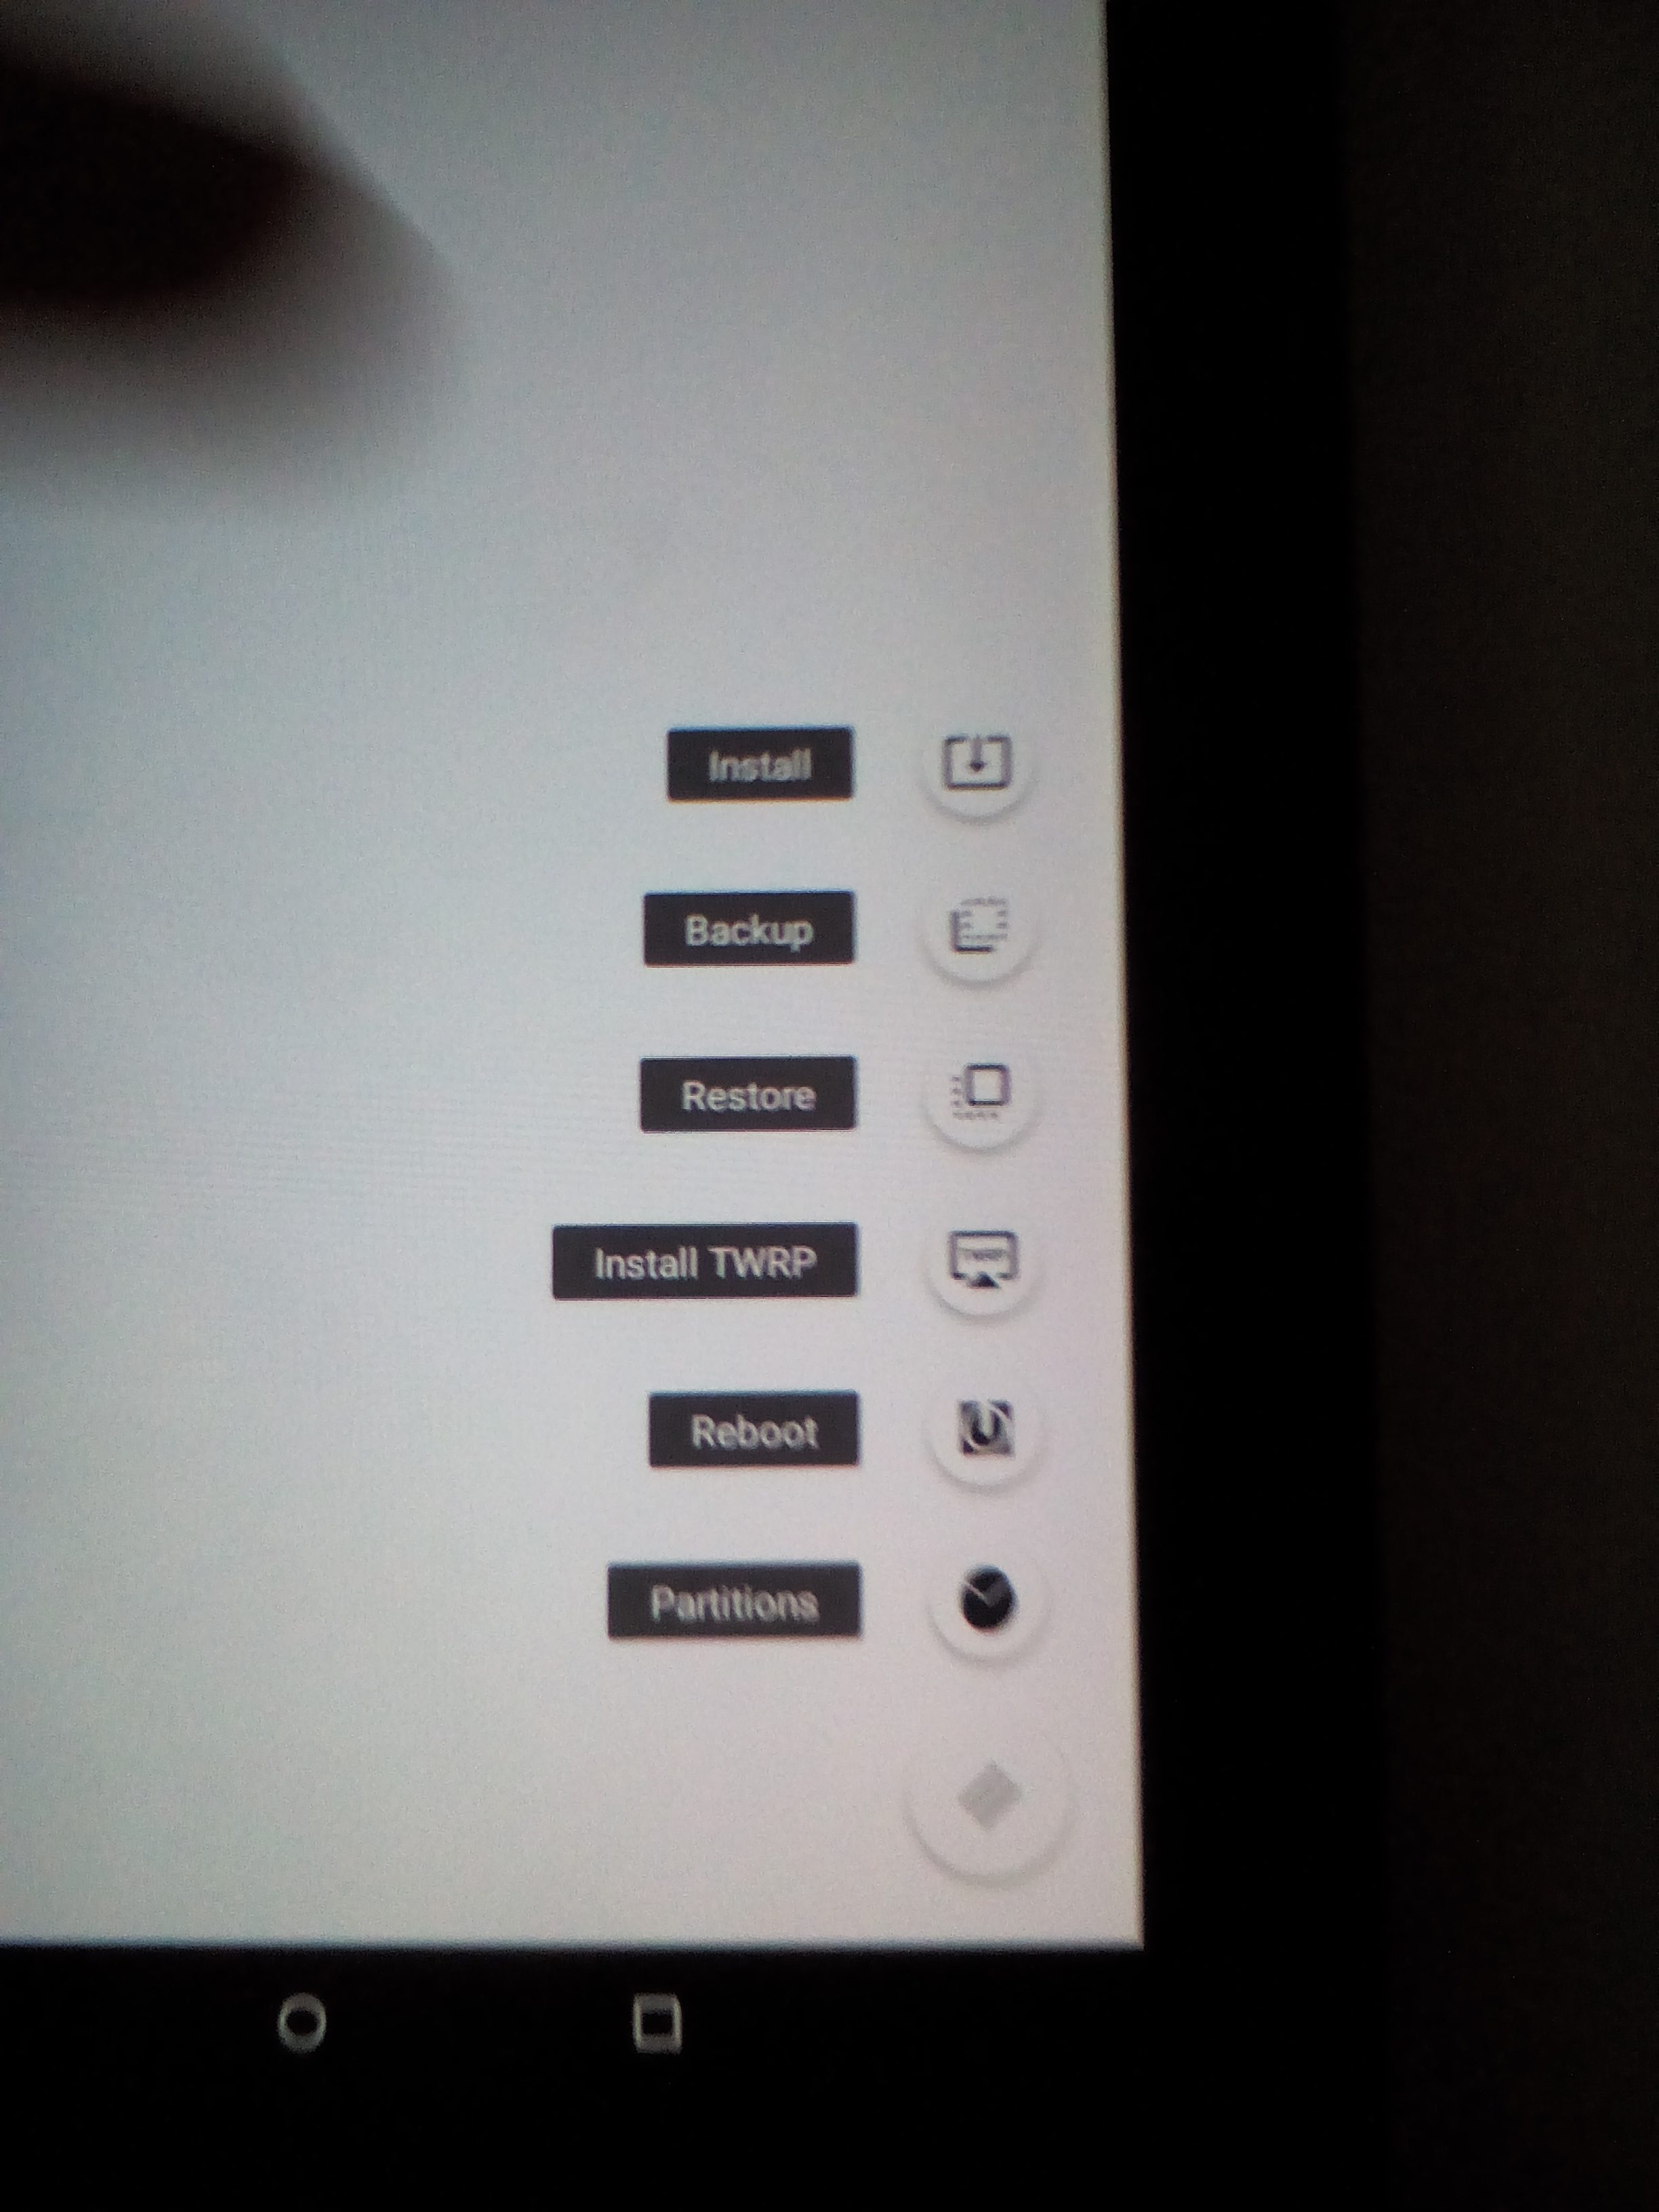
\includegraphics[scale=0.1]{./Image/img10}  \\
\caption{Backup}
\end{center}
\end{figure} 

\subsection{gerootetes Android-Tablet für diese Installation erforderlich}
Das Gerät muss gerootet sein. \\
"Root" unter Android ist ganz wichtig, fall etwas nicht gut passiert.

\subsection{BusyBox}
Die Virtuelle Maschine ist eine Software, die viele der Standard-Unix-Befehle, wie die GNU Core Utilities implementiert.
Sie ist automatisch installiert. \\

\subsection{Der Bootloader}
Der Bootloader8(bootstrap loader),) muss entsperrt sein.
Der Bootloader lädt weitere Teile des Betriebssystems, und stellt er sicher, dass alles richtig und vollständig

\subsection{Die administrativen Rechte durch SuperSU}
Die administrativen Rechte unter Android werden durch \textbf{SuperSU} geregelt.

\subsection{Die richtige Version von Kali Nethunter herunterladen}
Laden die richtige Version von Nethunter für Nexus 7 Android 5.1.1 herunter. Diese Version heißt \textbf{Lilopop} \\

Link: http://null-byte.wonderhowto.com/how-to/flash-kali-nethunter-oneplus-and-nexus-devices-most-as-secondary-rom-0162389/

\subsection{TWRP custom Recovery Installen}
Mit  "Team Win Recovery Project" (TWRP) können wir Custom-ROMs installieren und ein komplettes Backup unseres Android-Tablet erstellen. Außerdem hilft die Custom-Recovery beim rooten unseres Smartphones.

Schauen die Figure 8 und 9 an, wie TWRP aussieht, sein Version und Kontakt. \\

\begin{figure}[H]
\begin{center} 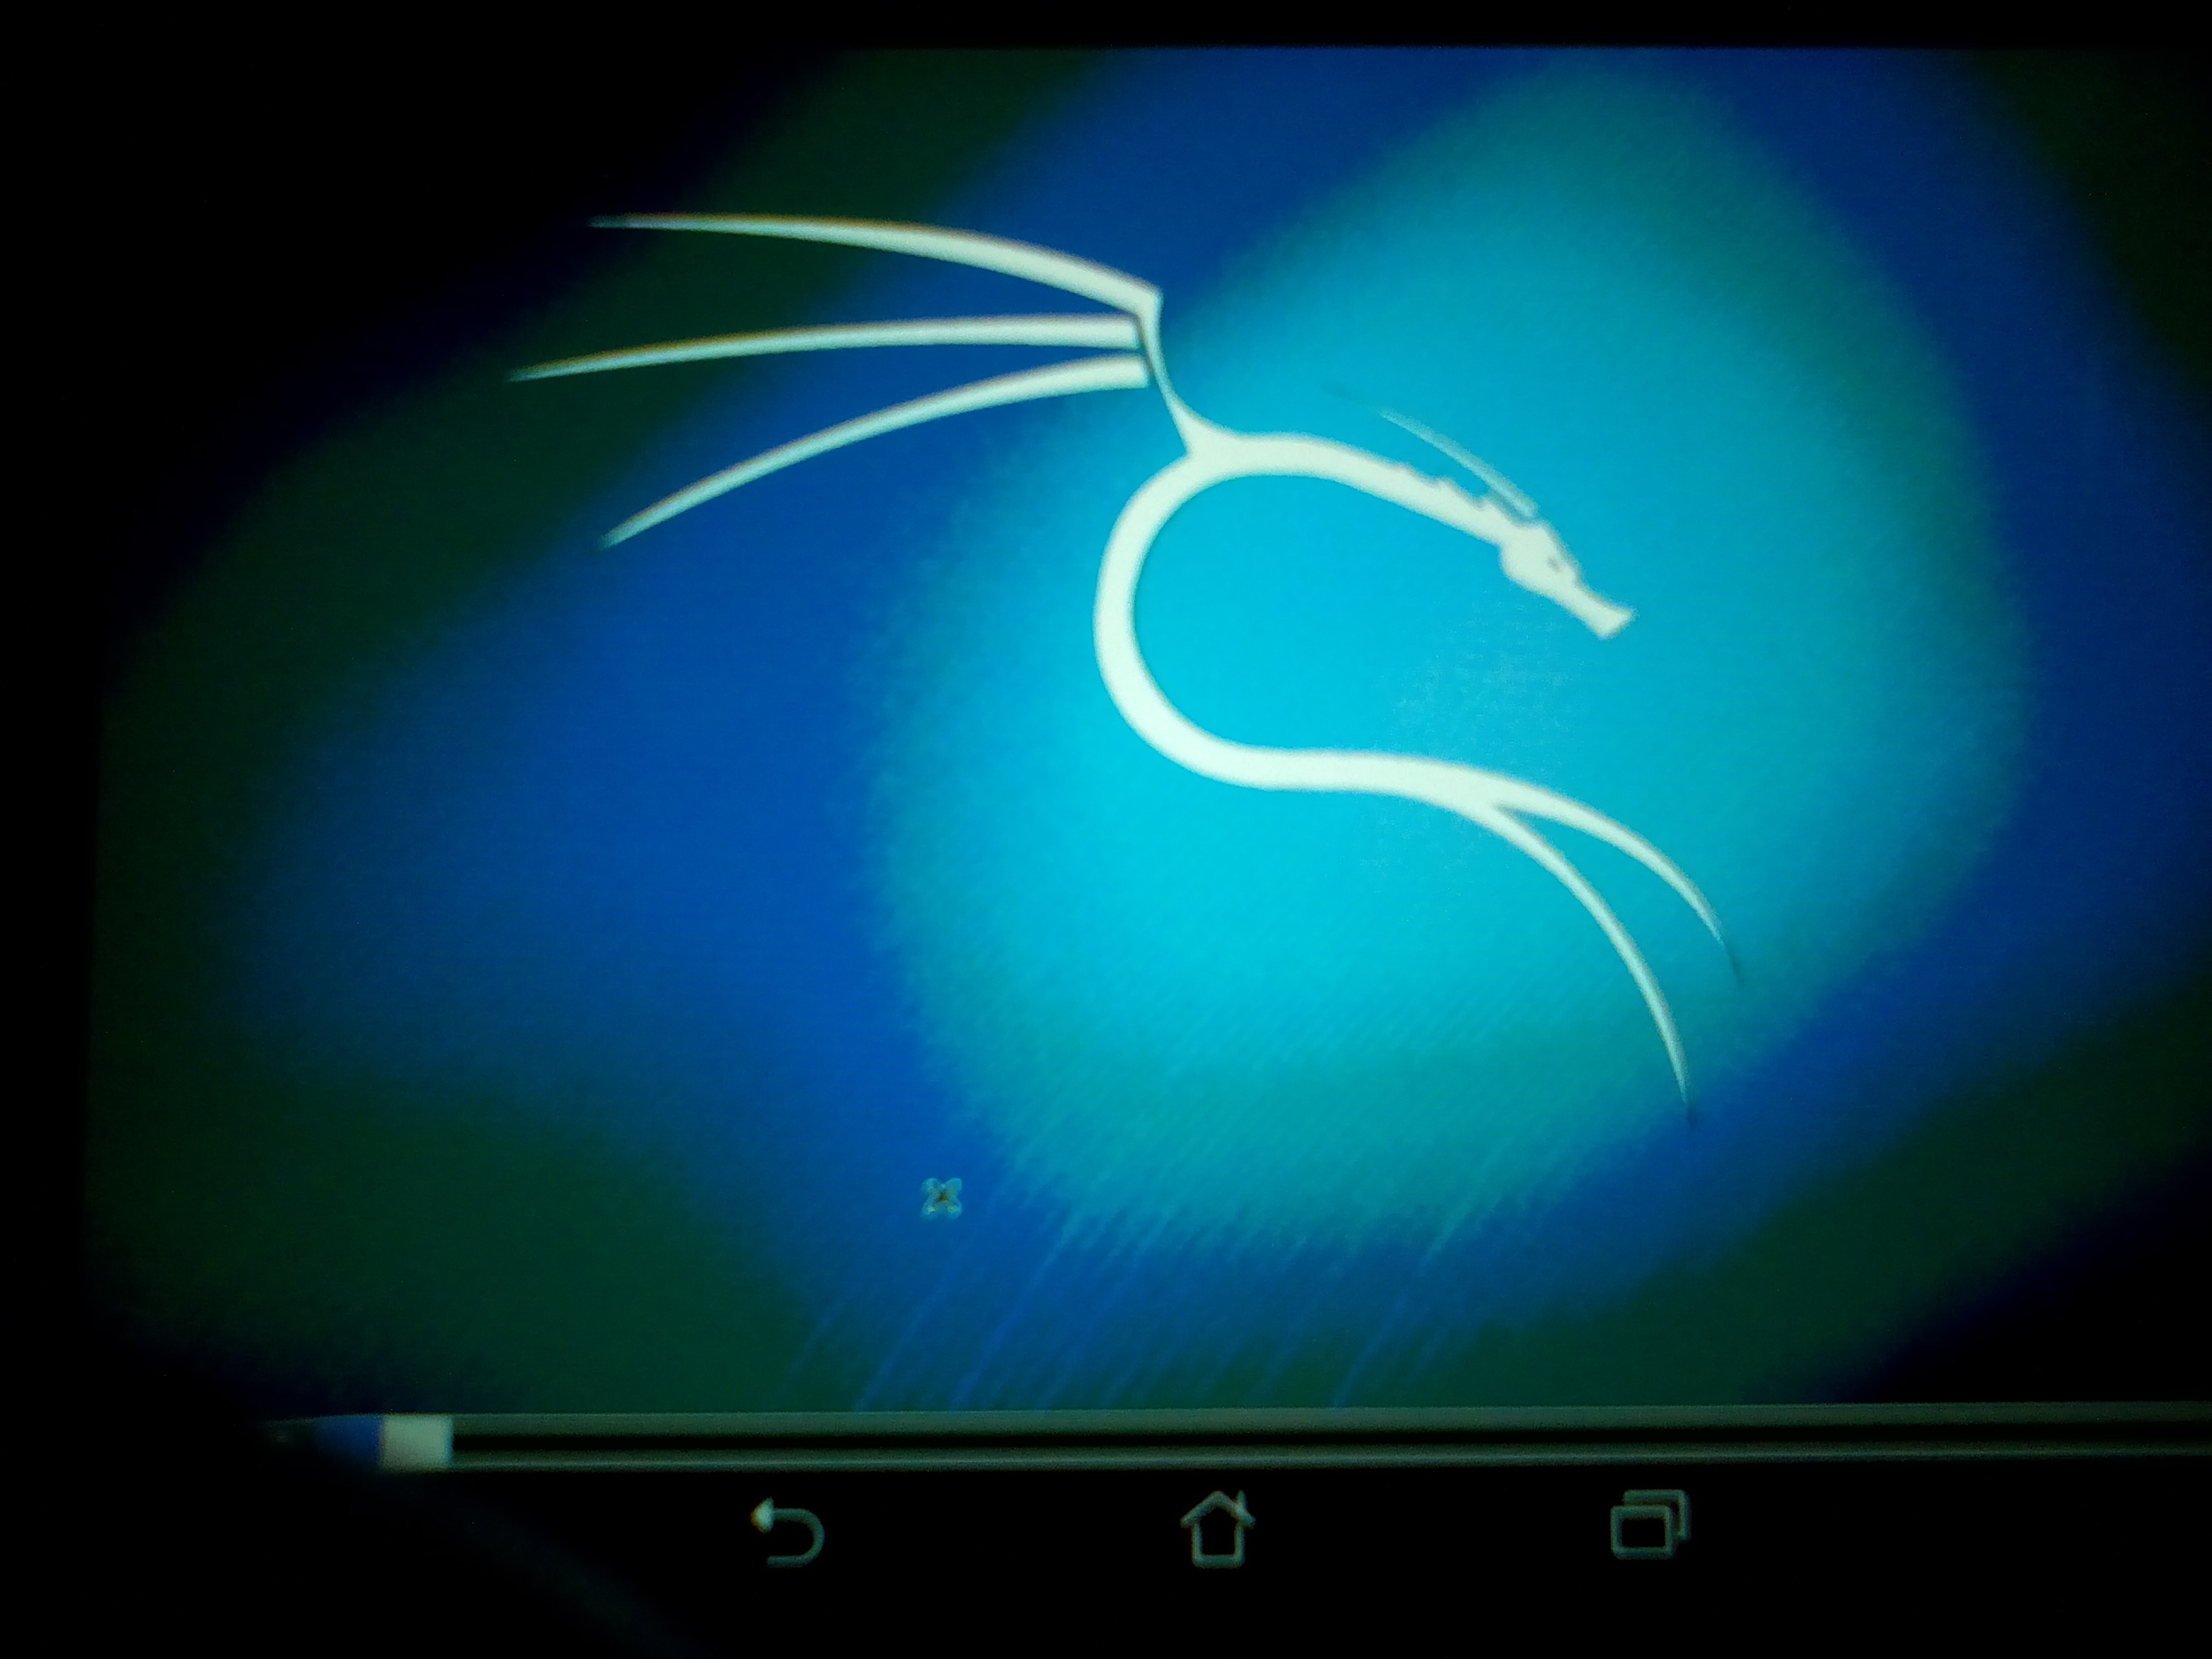
\includegraphics[scale=0.1]{./Image/img8}  \\
\caption{TWRP}
\end{center}
\end{figure} 

\begin{figure}[H]
\begin{center} 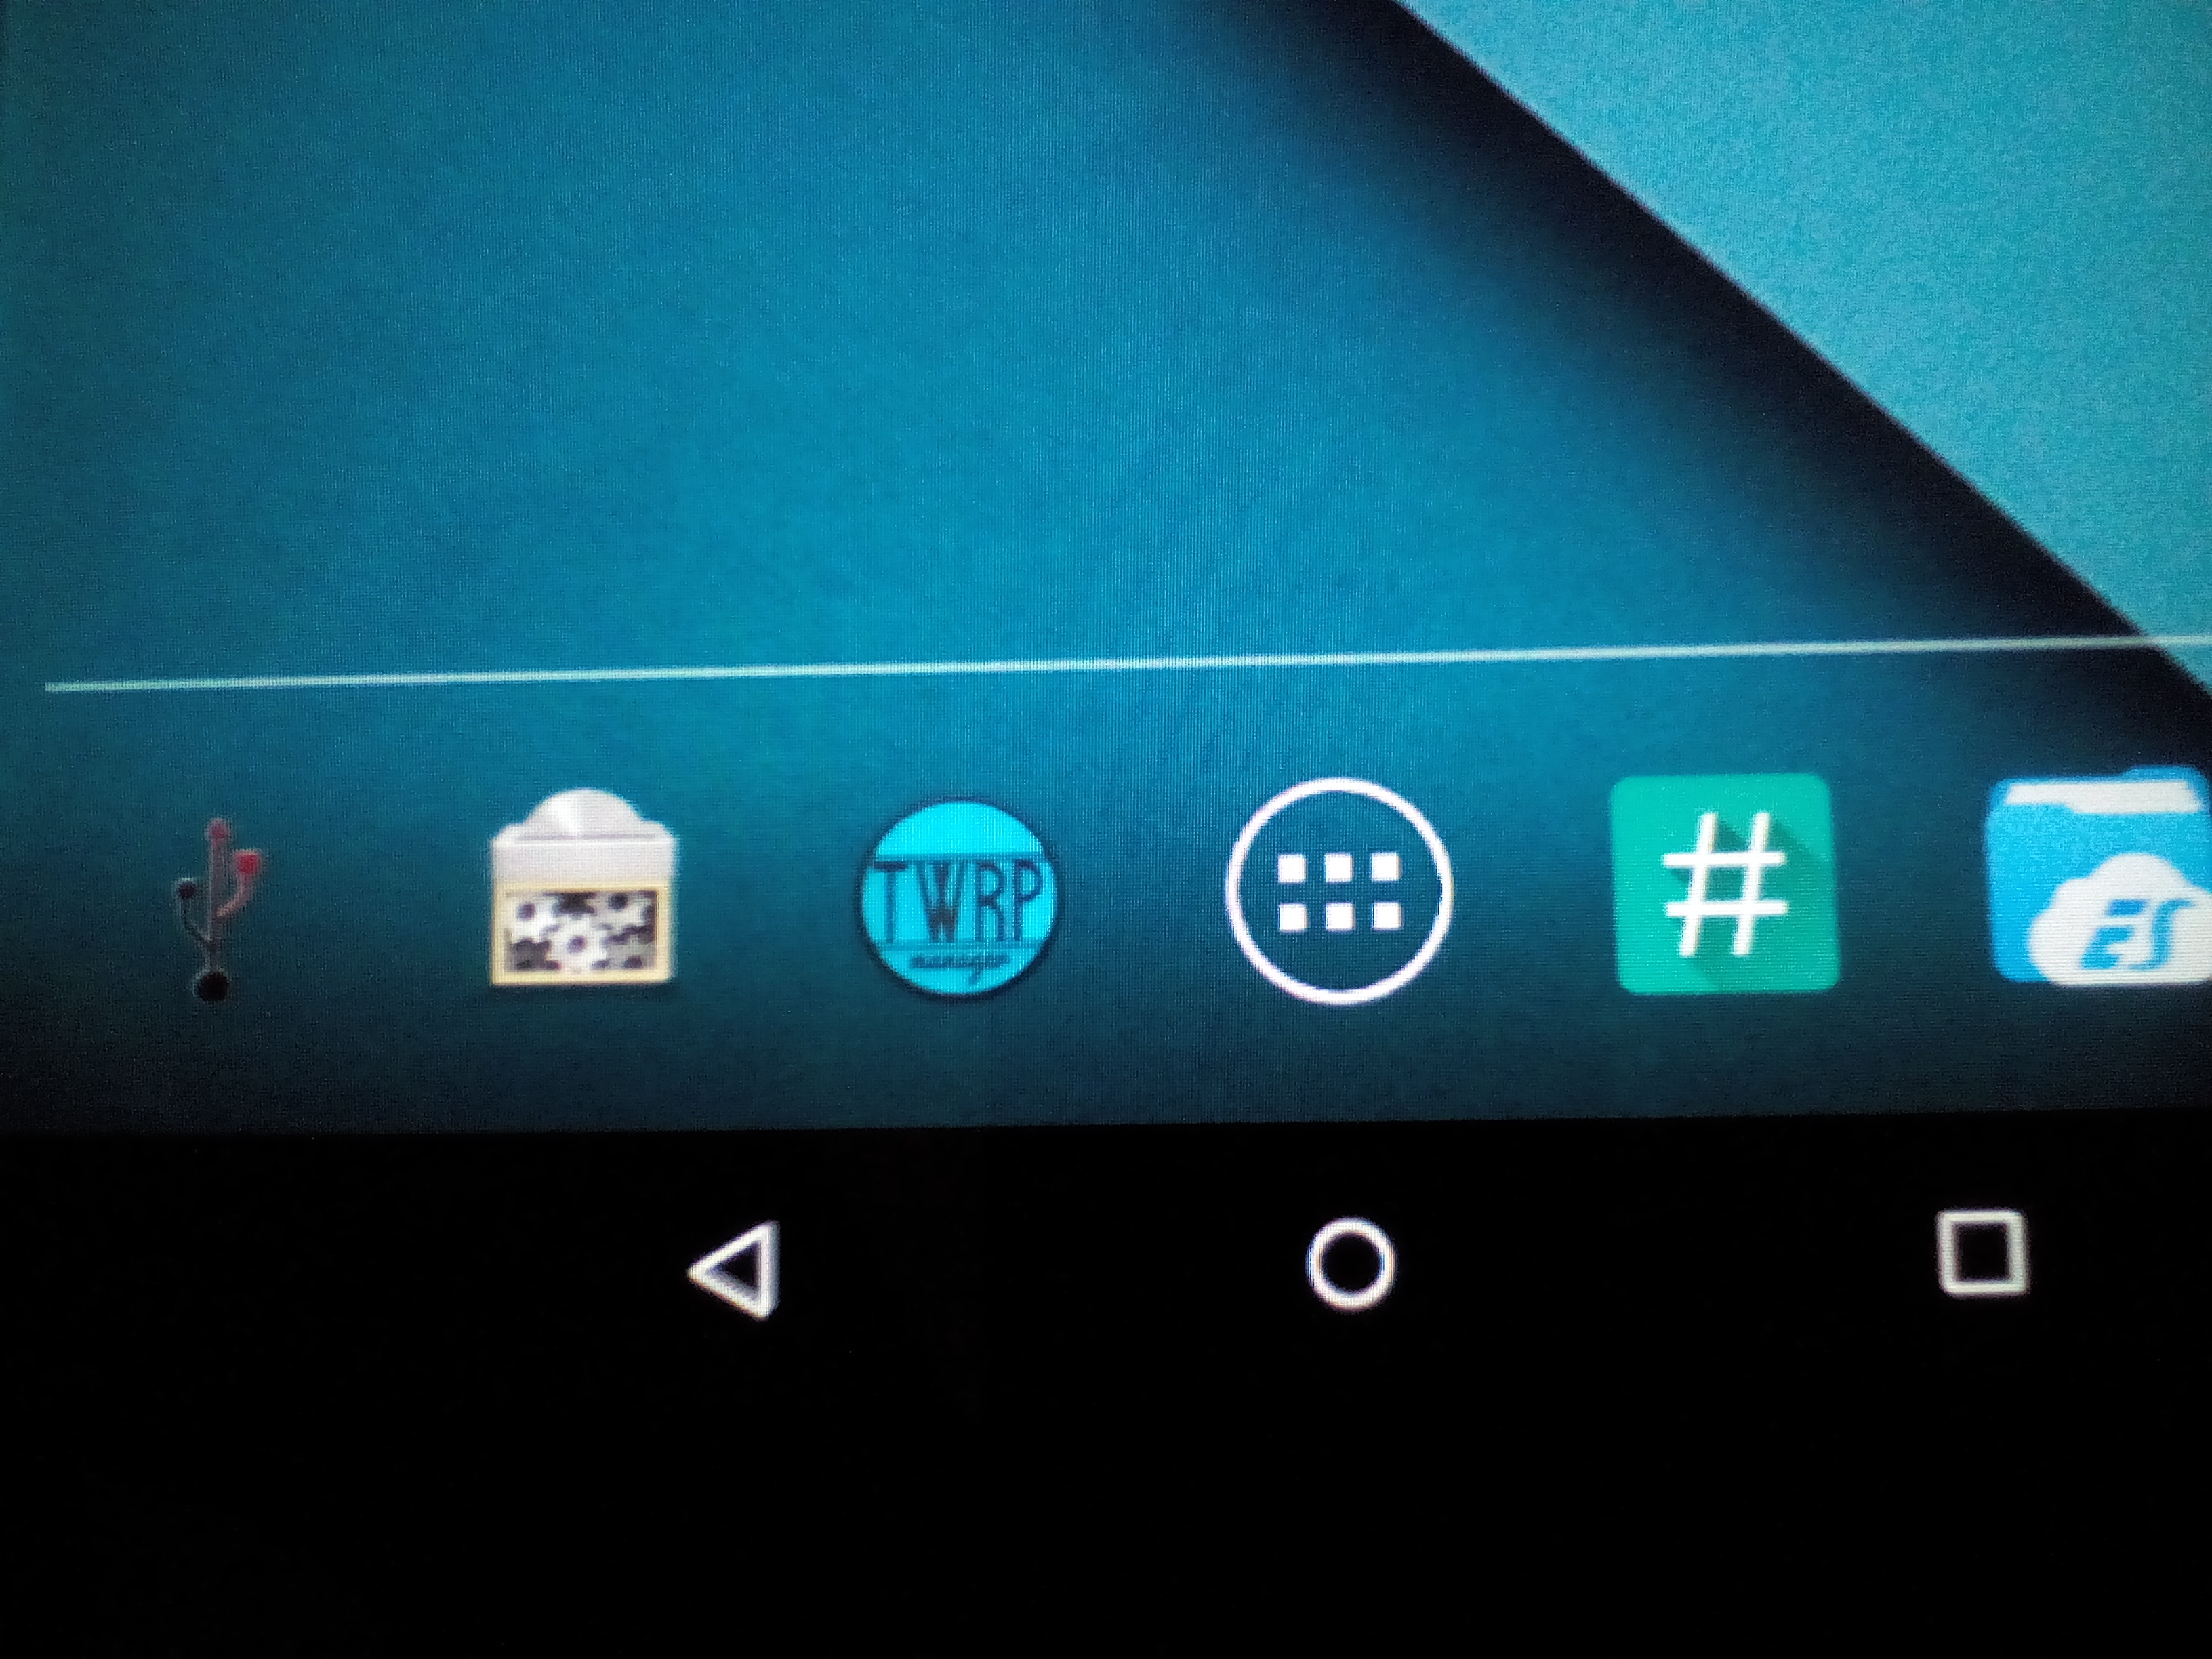
\includegraphics[scale=0.1]{./Image/img9}  \\
\caption{TWRP Version und Kontakt}
\end{center}
\end{figure} 

TWRP bietet eine höhe Verfugbarkeit die Virtuelle Maschine an. Wir klicken dann darauf (High Availability für die Virtuelle Maschine)\\

Die Figure 11 zeigt das.

\begin{figure}[H]
\begin{center} 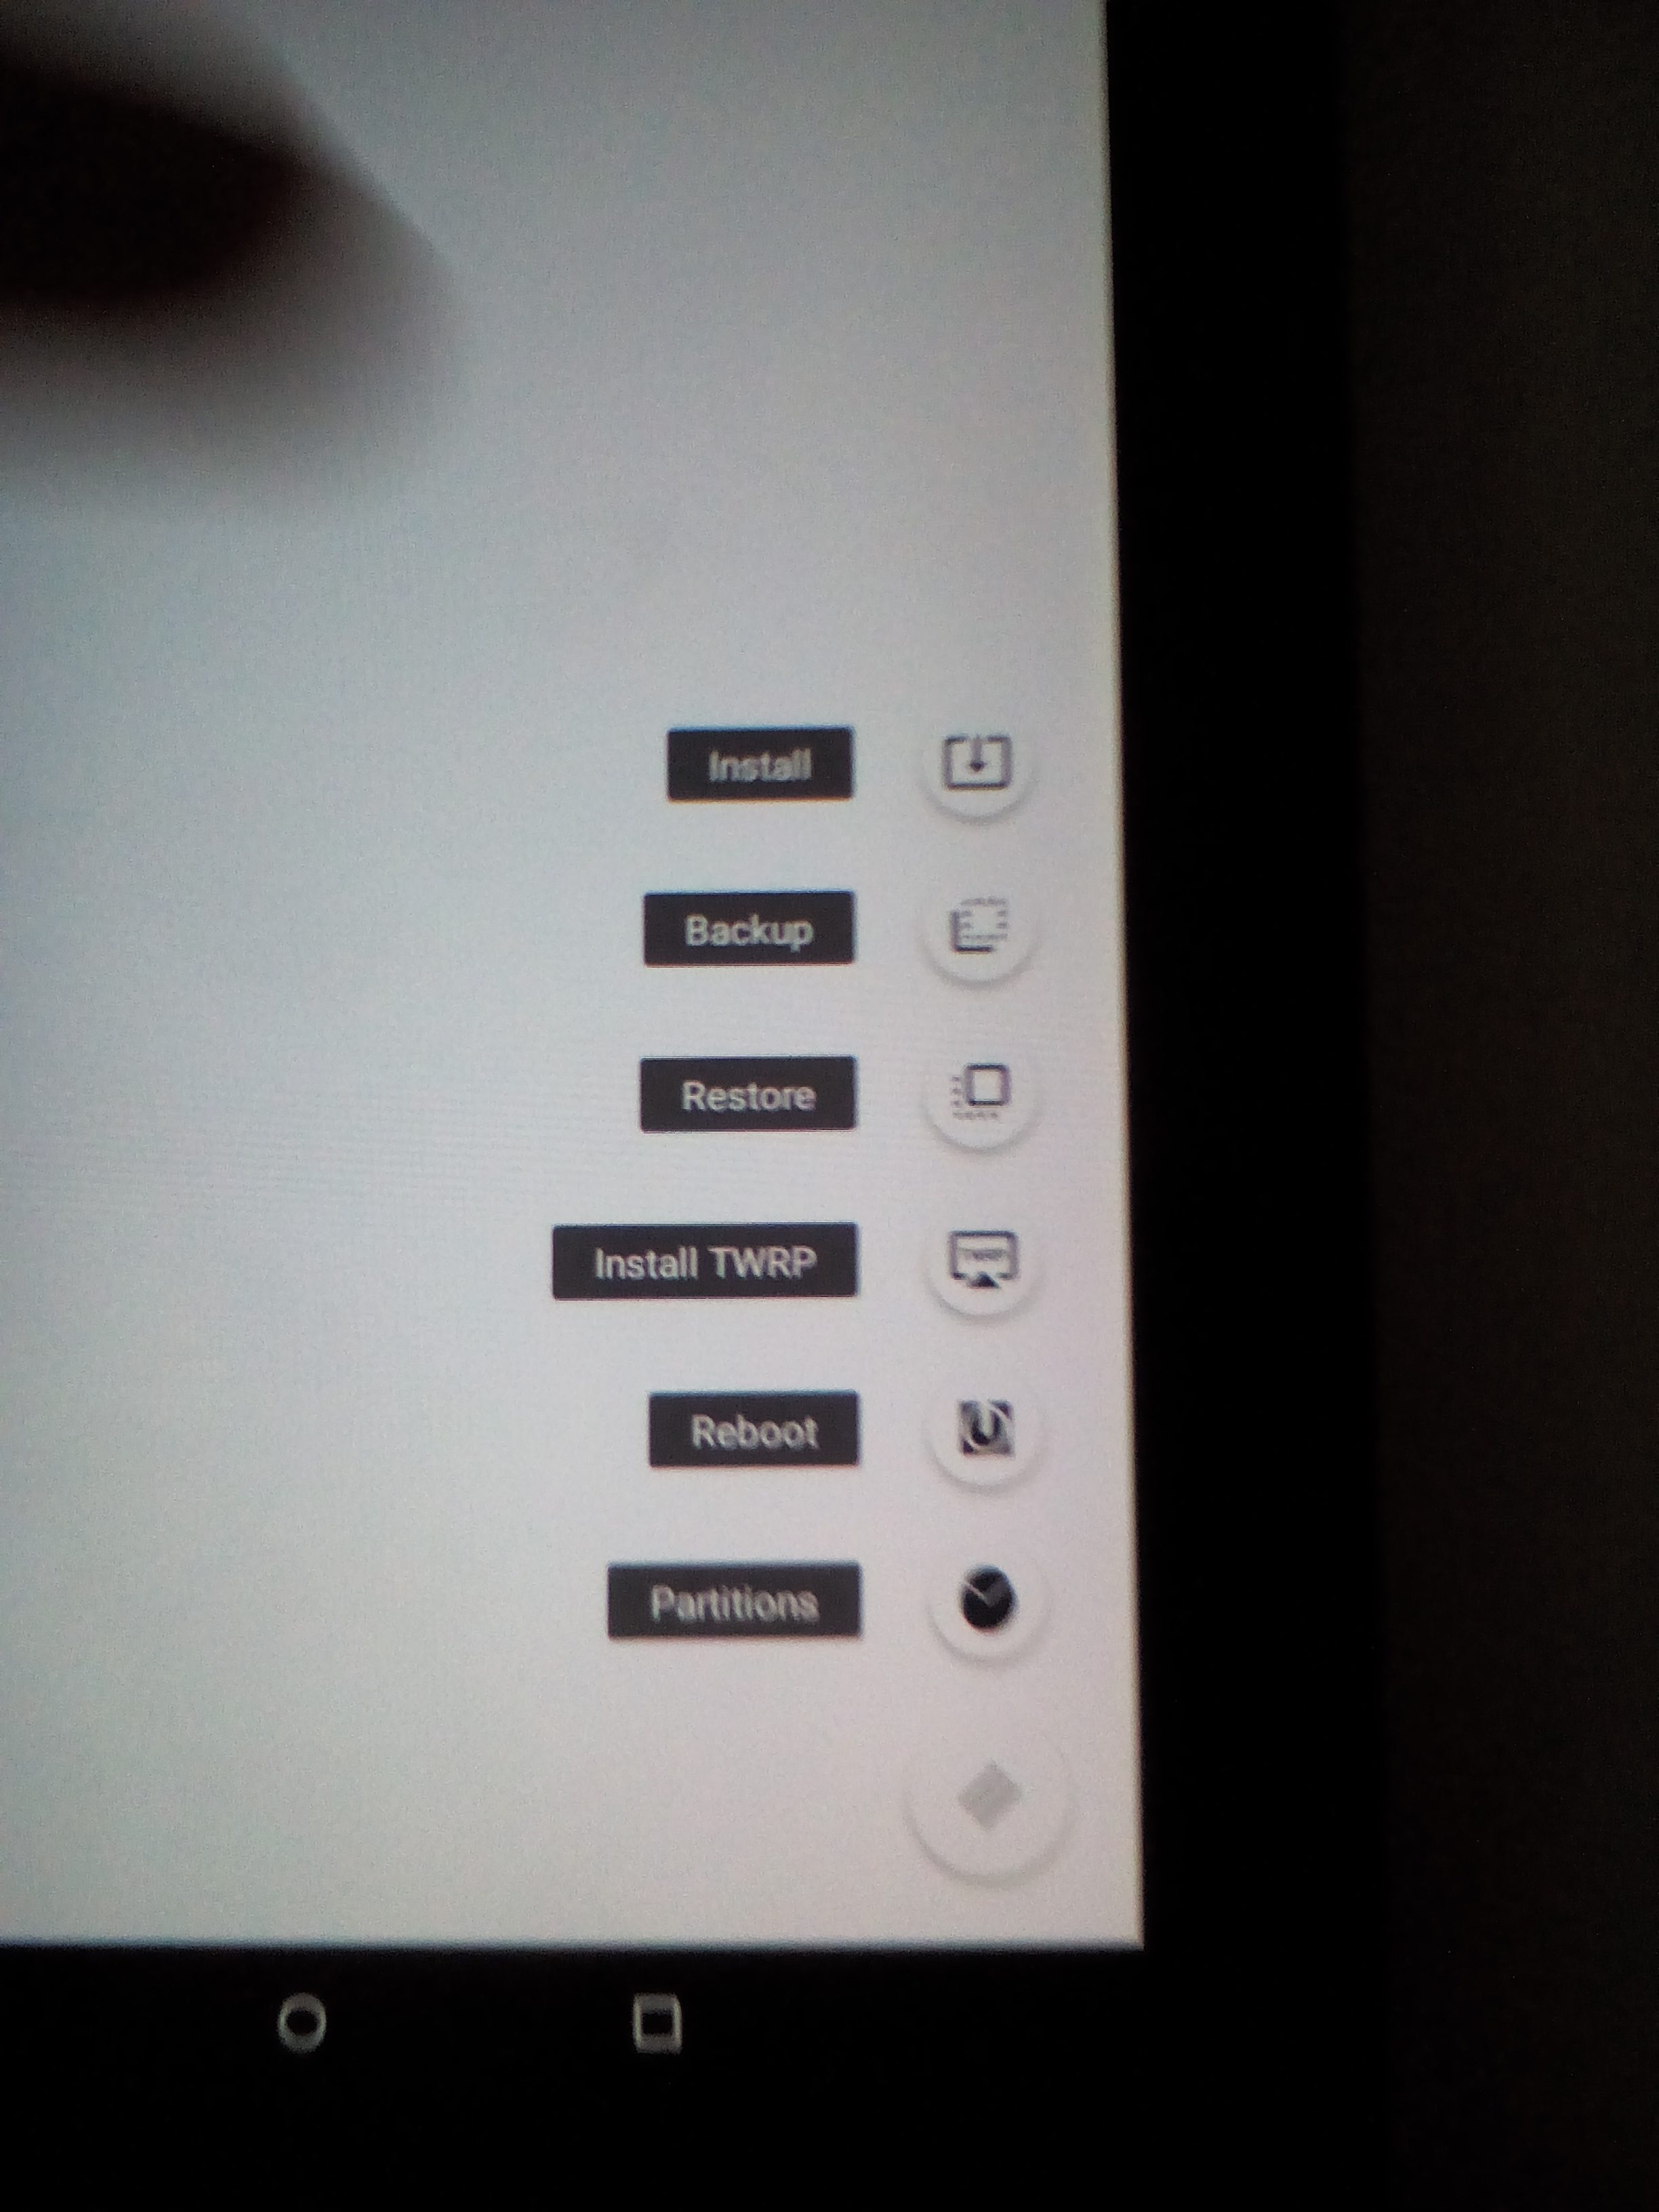
\includegraphics[scale=0.1]{./Image/img11}  \\
\caption{Höhe Verfugbarkeit}
\end{center}
\end{figure} 

Wir sehen dann ein Warning Message (Figure 12)\\
Nichts Schlimmes.
Nethunter installiert und verwendet Standard-Kali-Distribution. Um diese Funktionalität zu unterstützen, sind einige Standard-Android-Sicherheitsfunktionen deaktiviert. \\

\begin{figure}[H]
\begin{center} 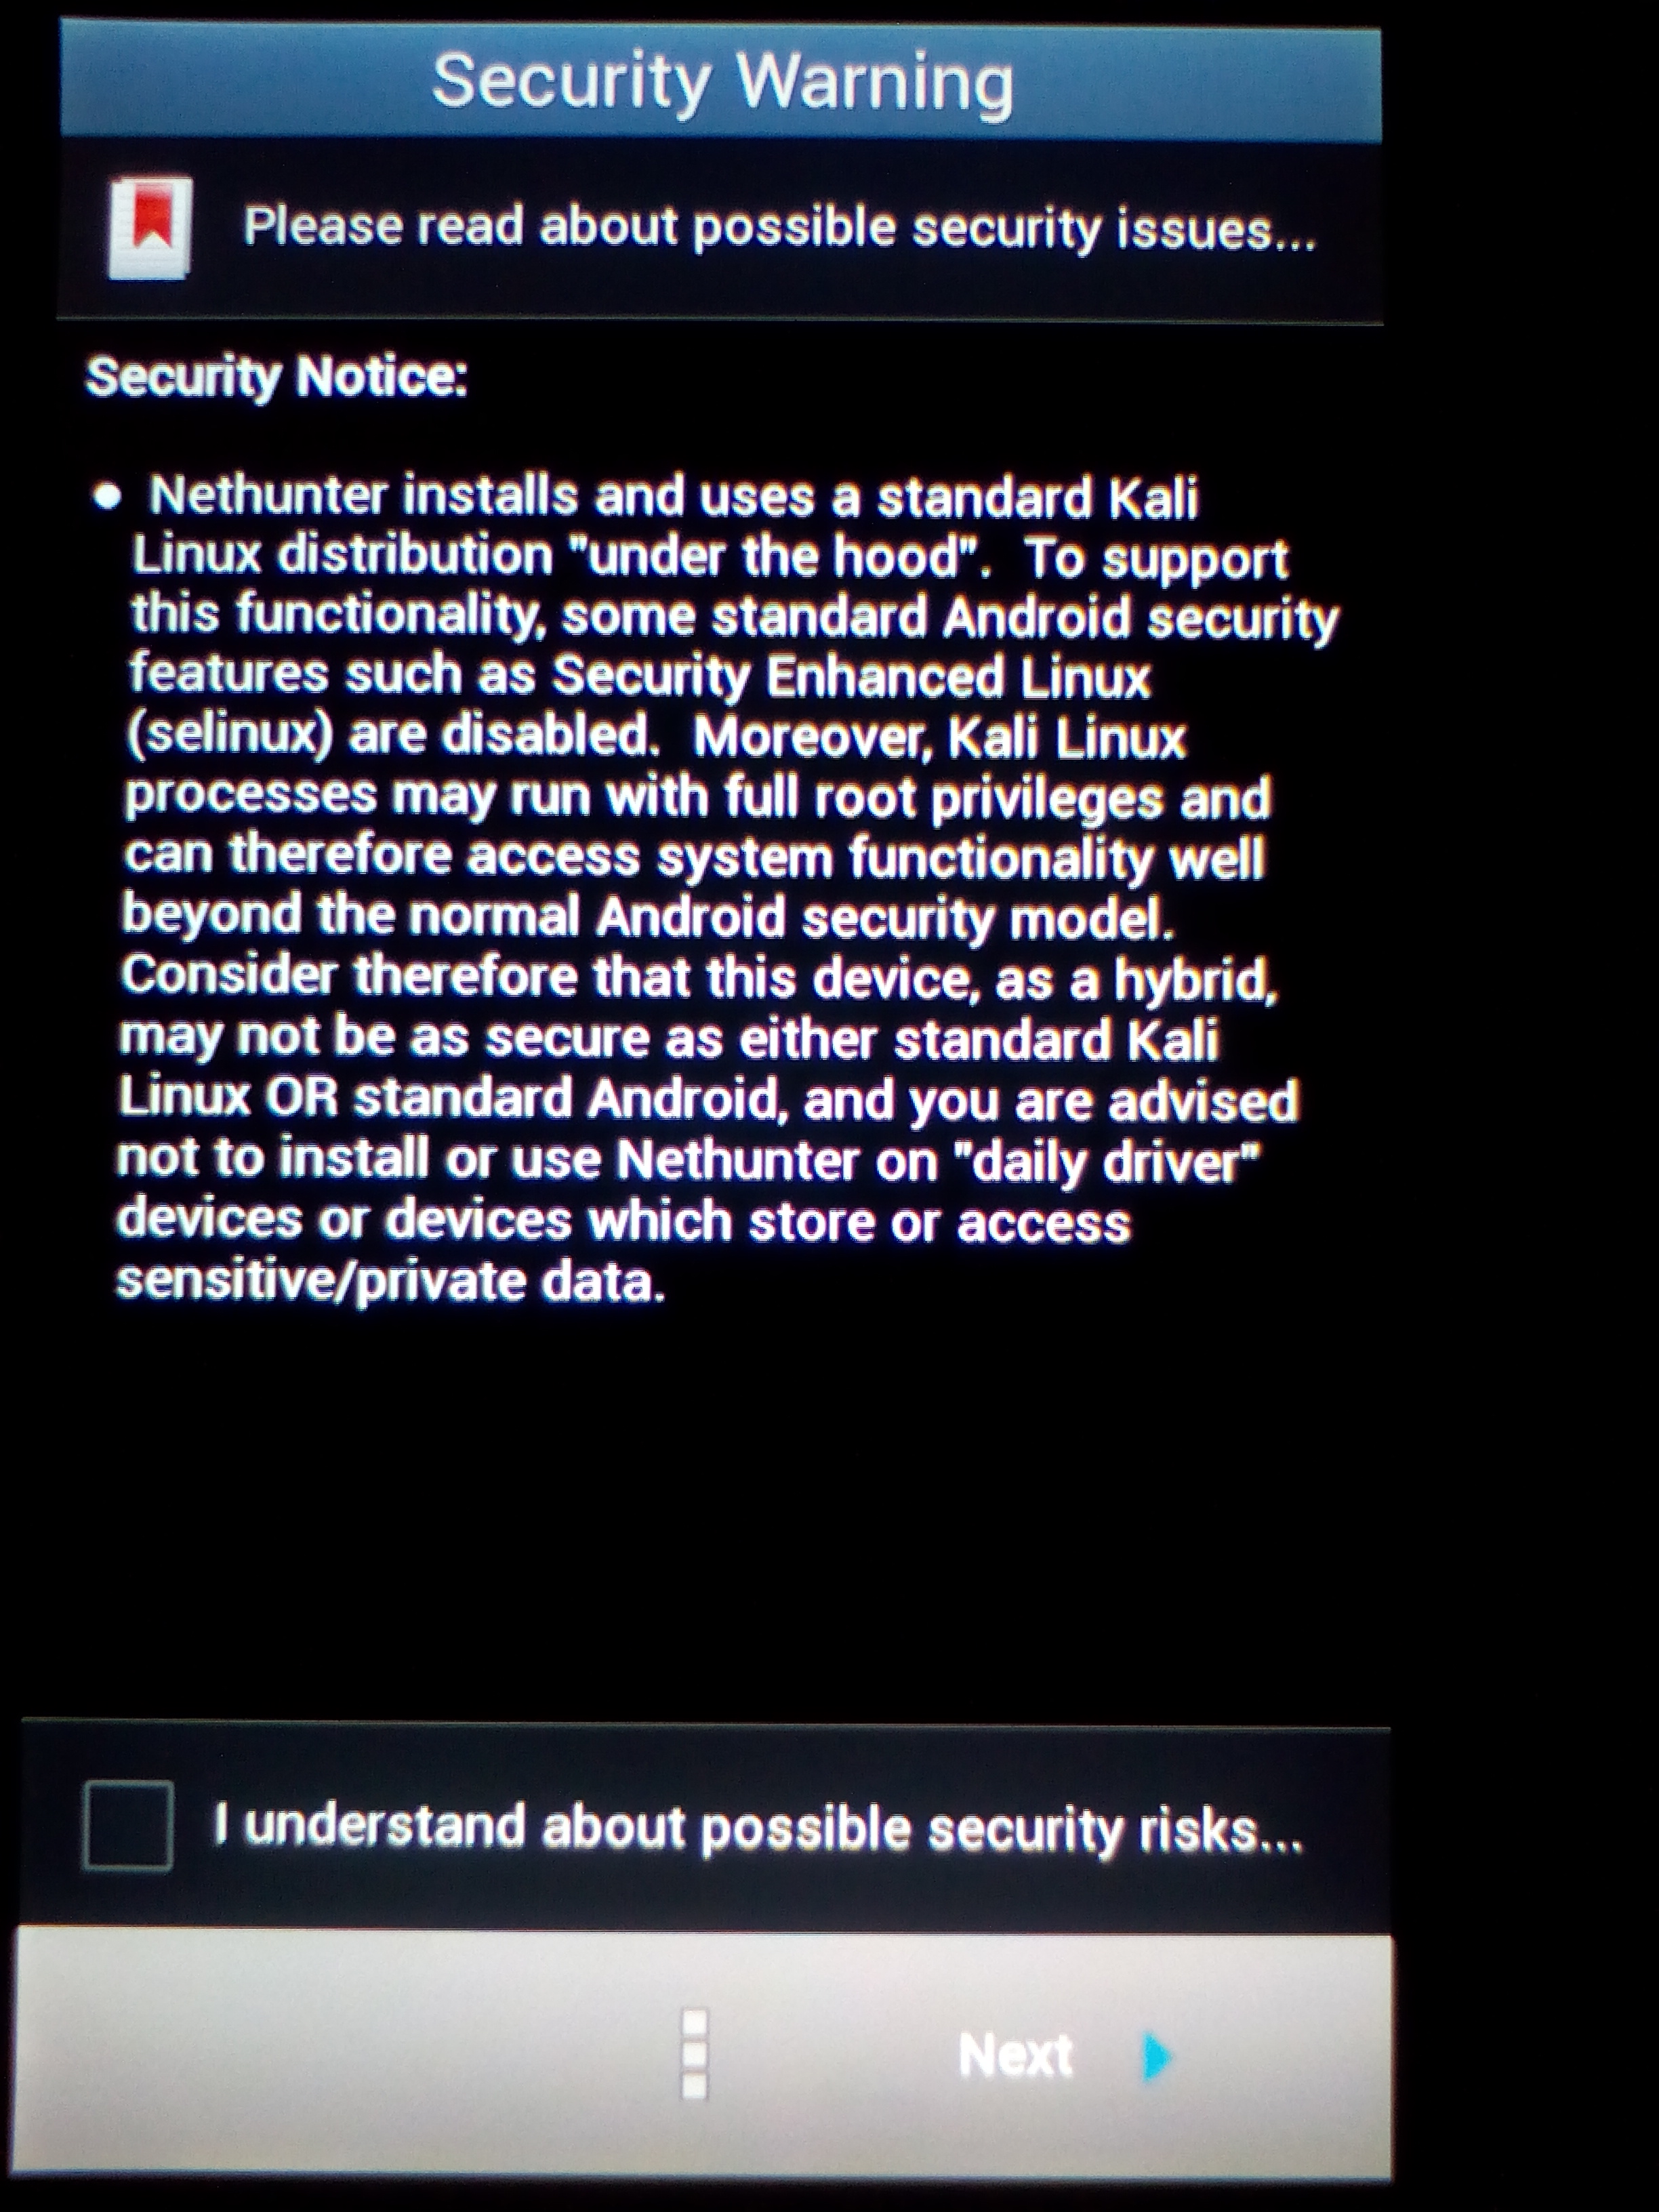
\includegraphics[scale=0.1]{./Image/img12}  \\
\caption{Warning}
\end{center}
\end{figure} 

Dann wir wählen die App zu installieren. \\
Anschauen Figure 13 \\

\begin{figure}[H]
\begin{center} 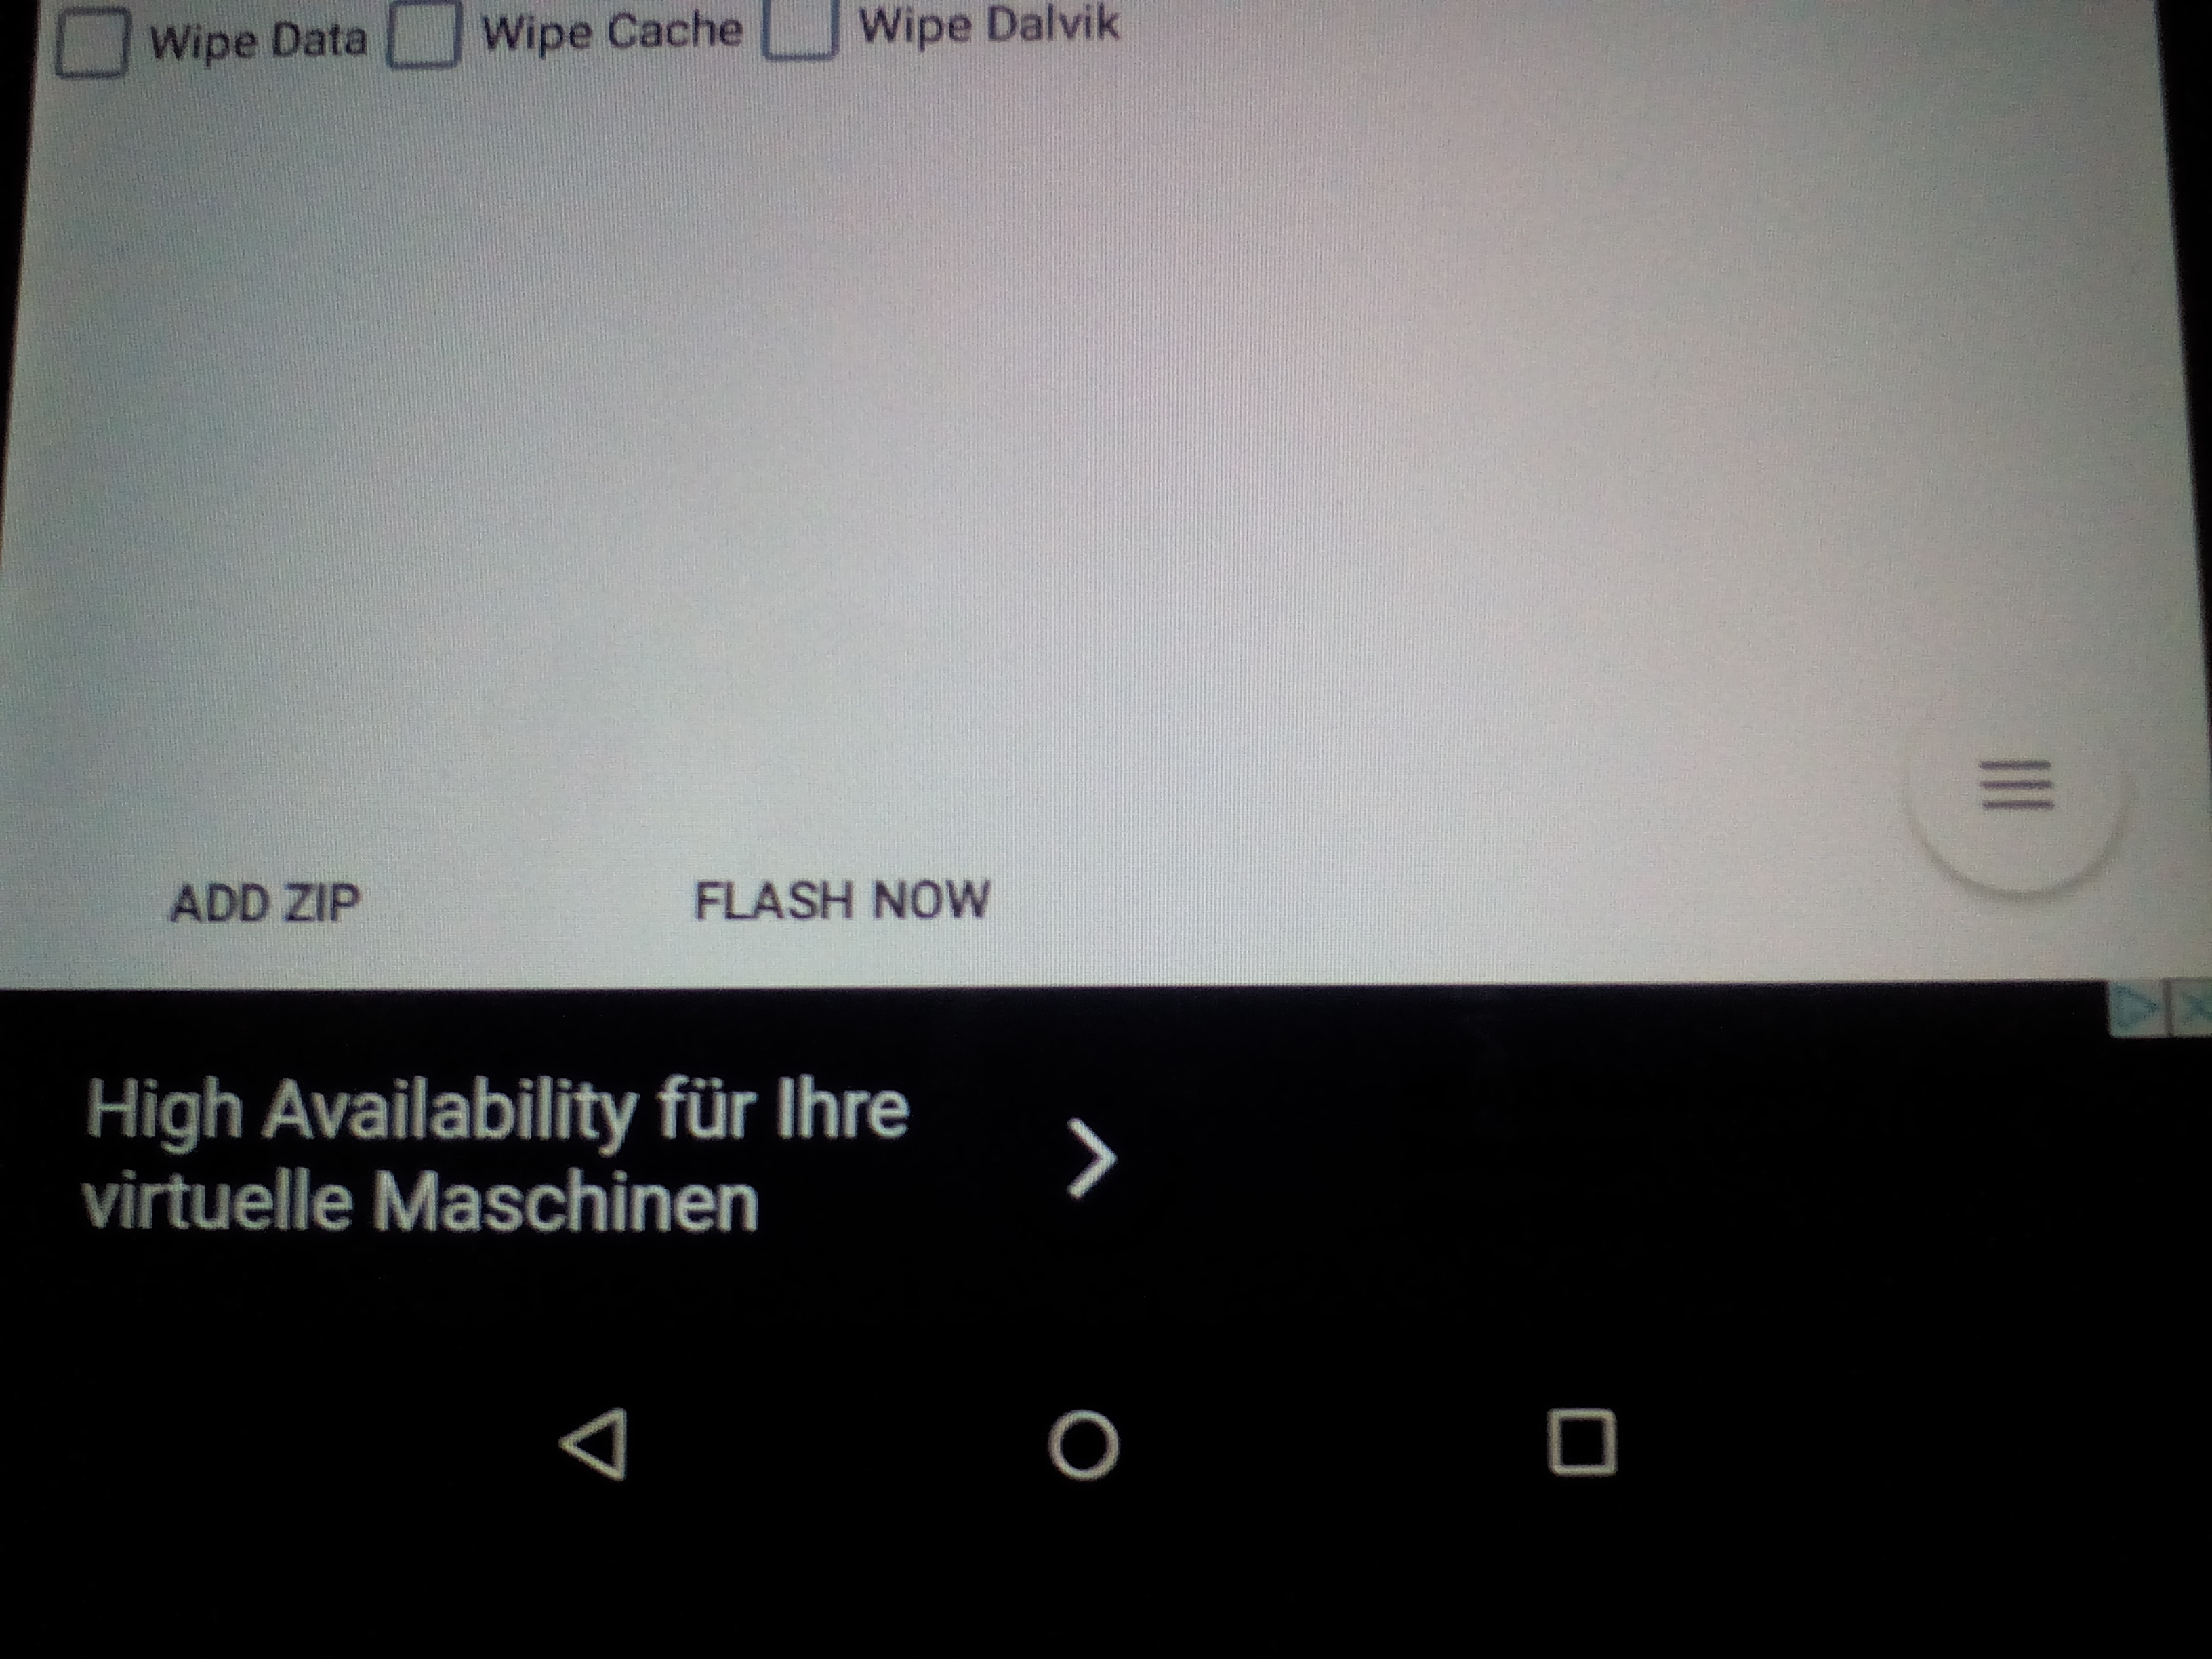
\includegraphics[scale=0.1]{./Image/img13}  \\
\caption{Auswahl der App}
\end{center}
\end{figure} 

Dann wir wählen die App zu installieren. \\
Diese Anwendungen sind: \\
- Nethunter \\
- Custom Nethunter Terminal Emulator \\
- Custom Nethunter VNC \\
- BlueNMEA \\
- drivedroid \\
- Hackerskeyboard \\
- RF-Analyser \\
- USB-Keyboard \\
- Router Keygen \\

Anschauen Figure 14 und 15\\

\begin{figure}[H]
\begin{center} 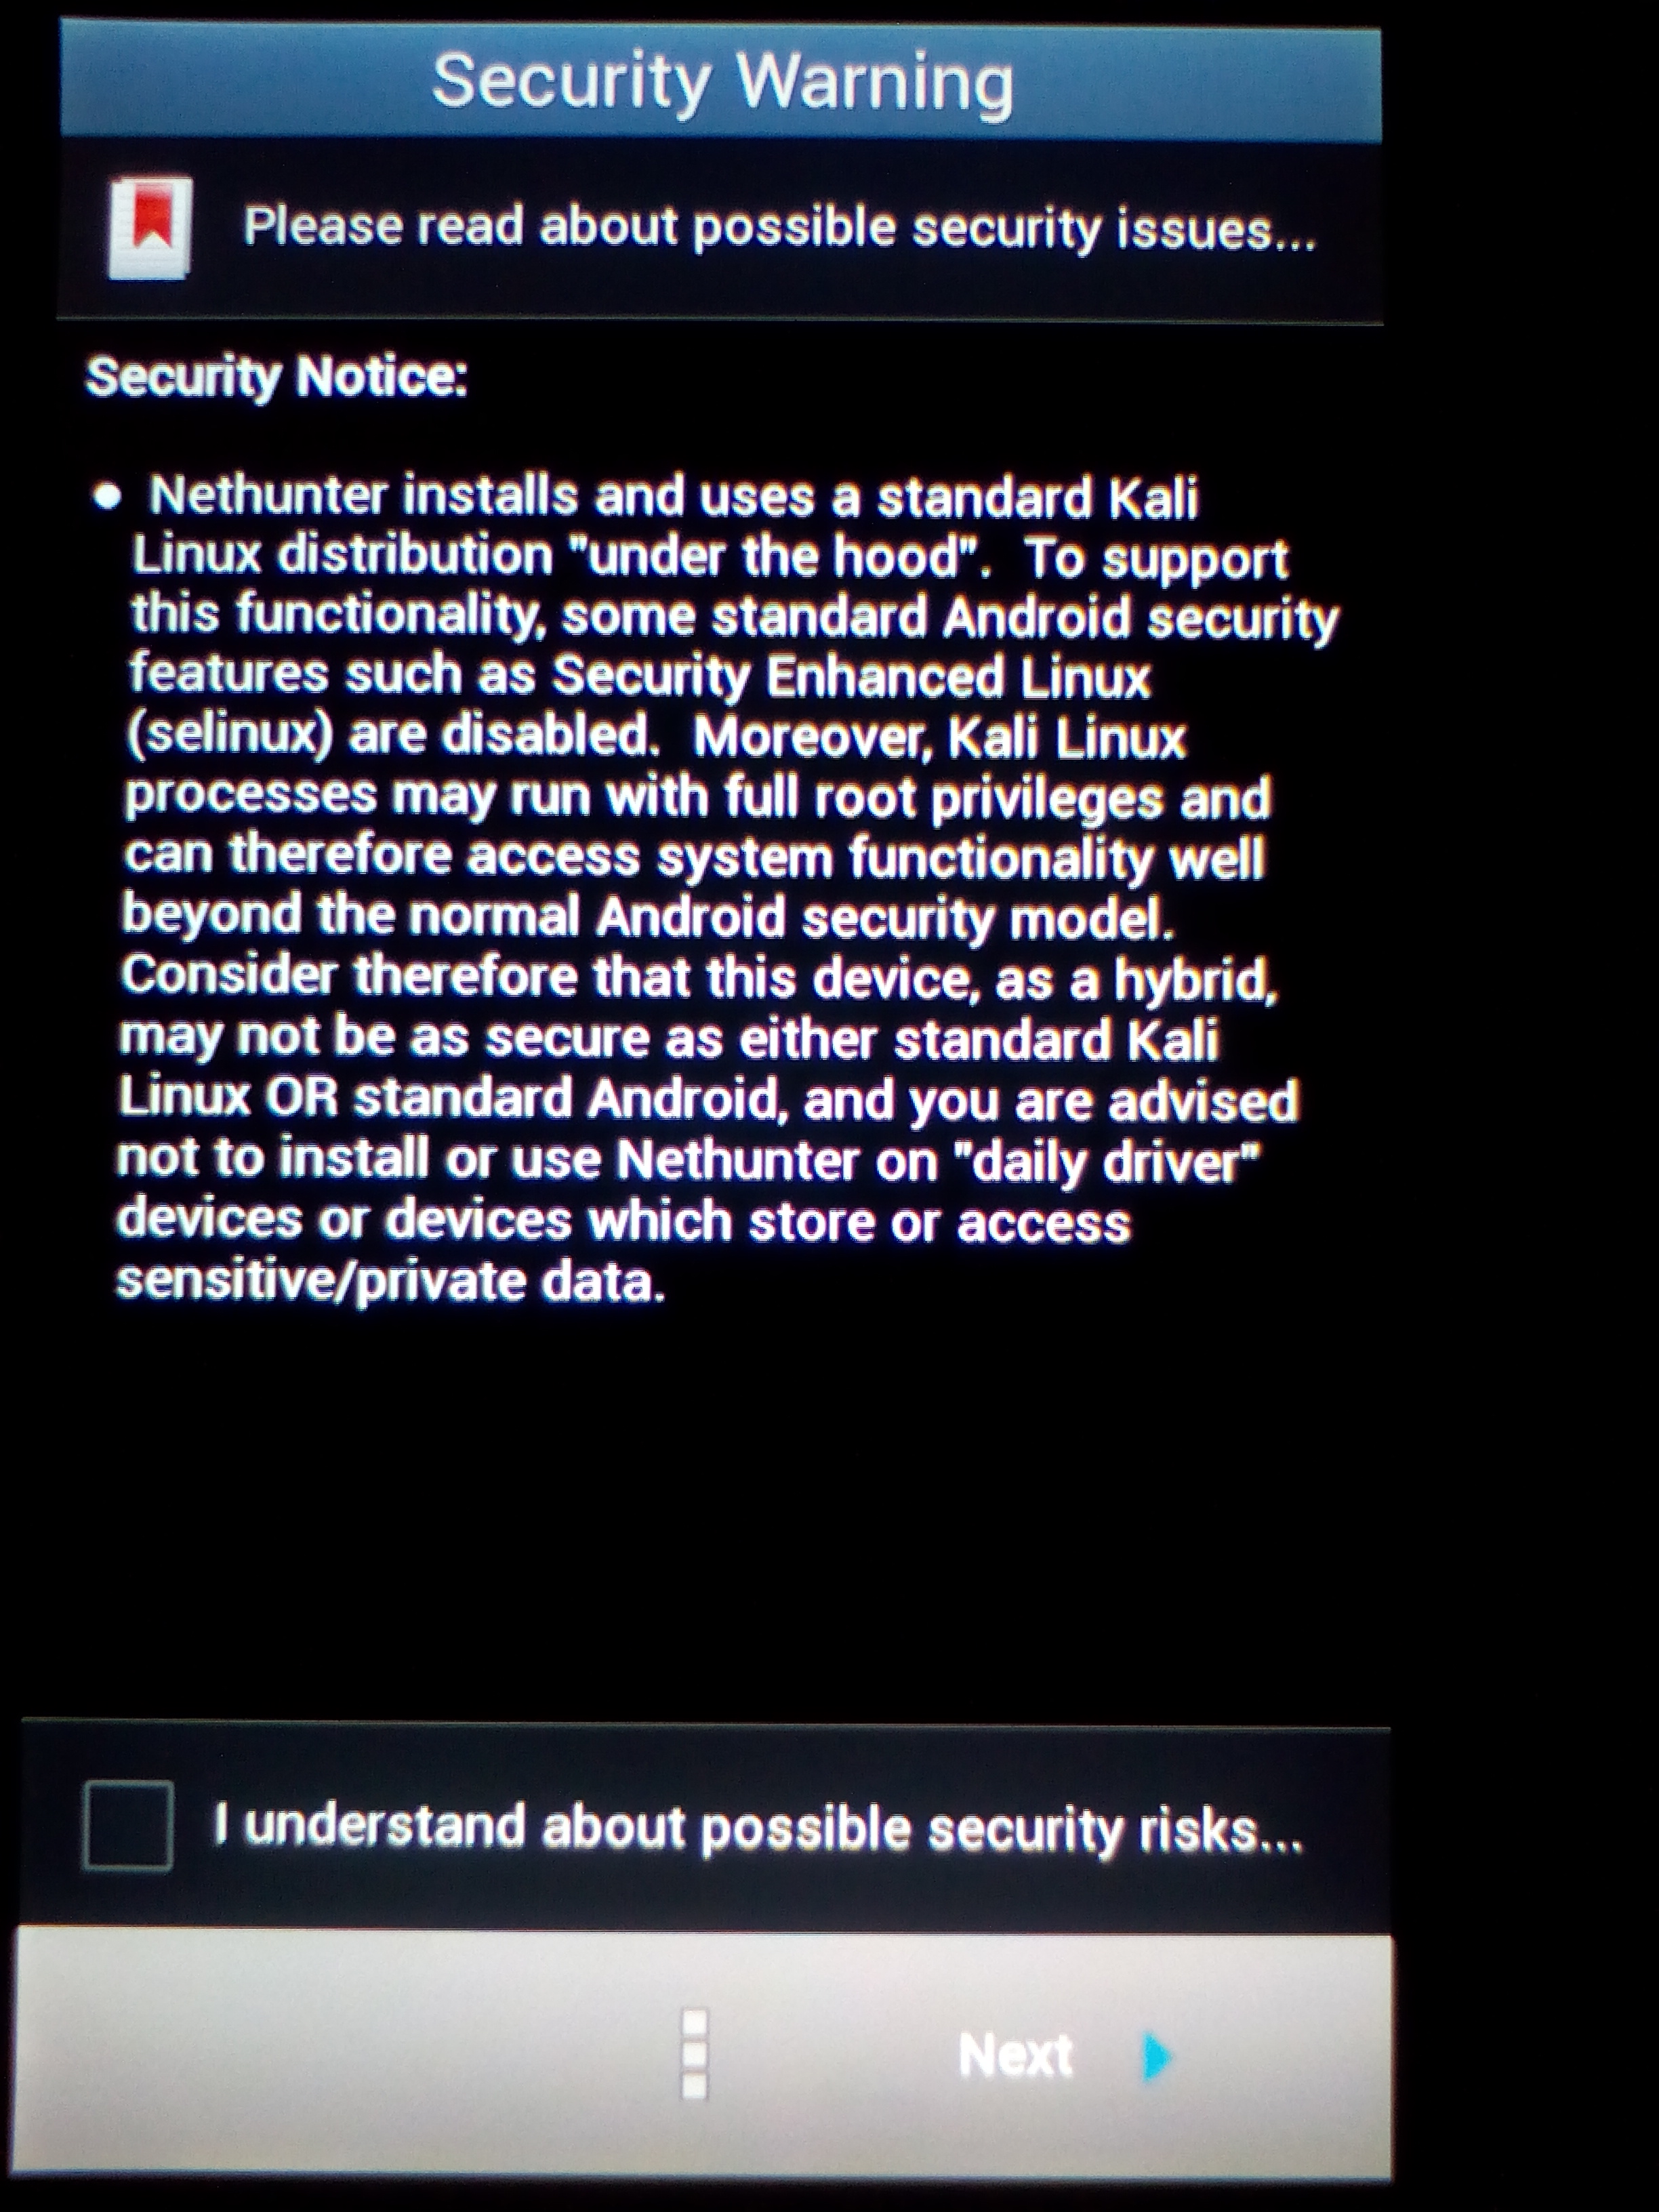
\includegraphics[scale=0.1]{./Image/img14}  \\
\caption{Anwendungen 1}
\end{center}
\end{figure} 


\begin{figure}[H]
\begin{center} 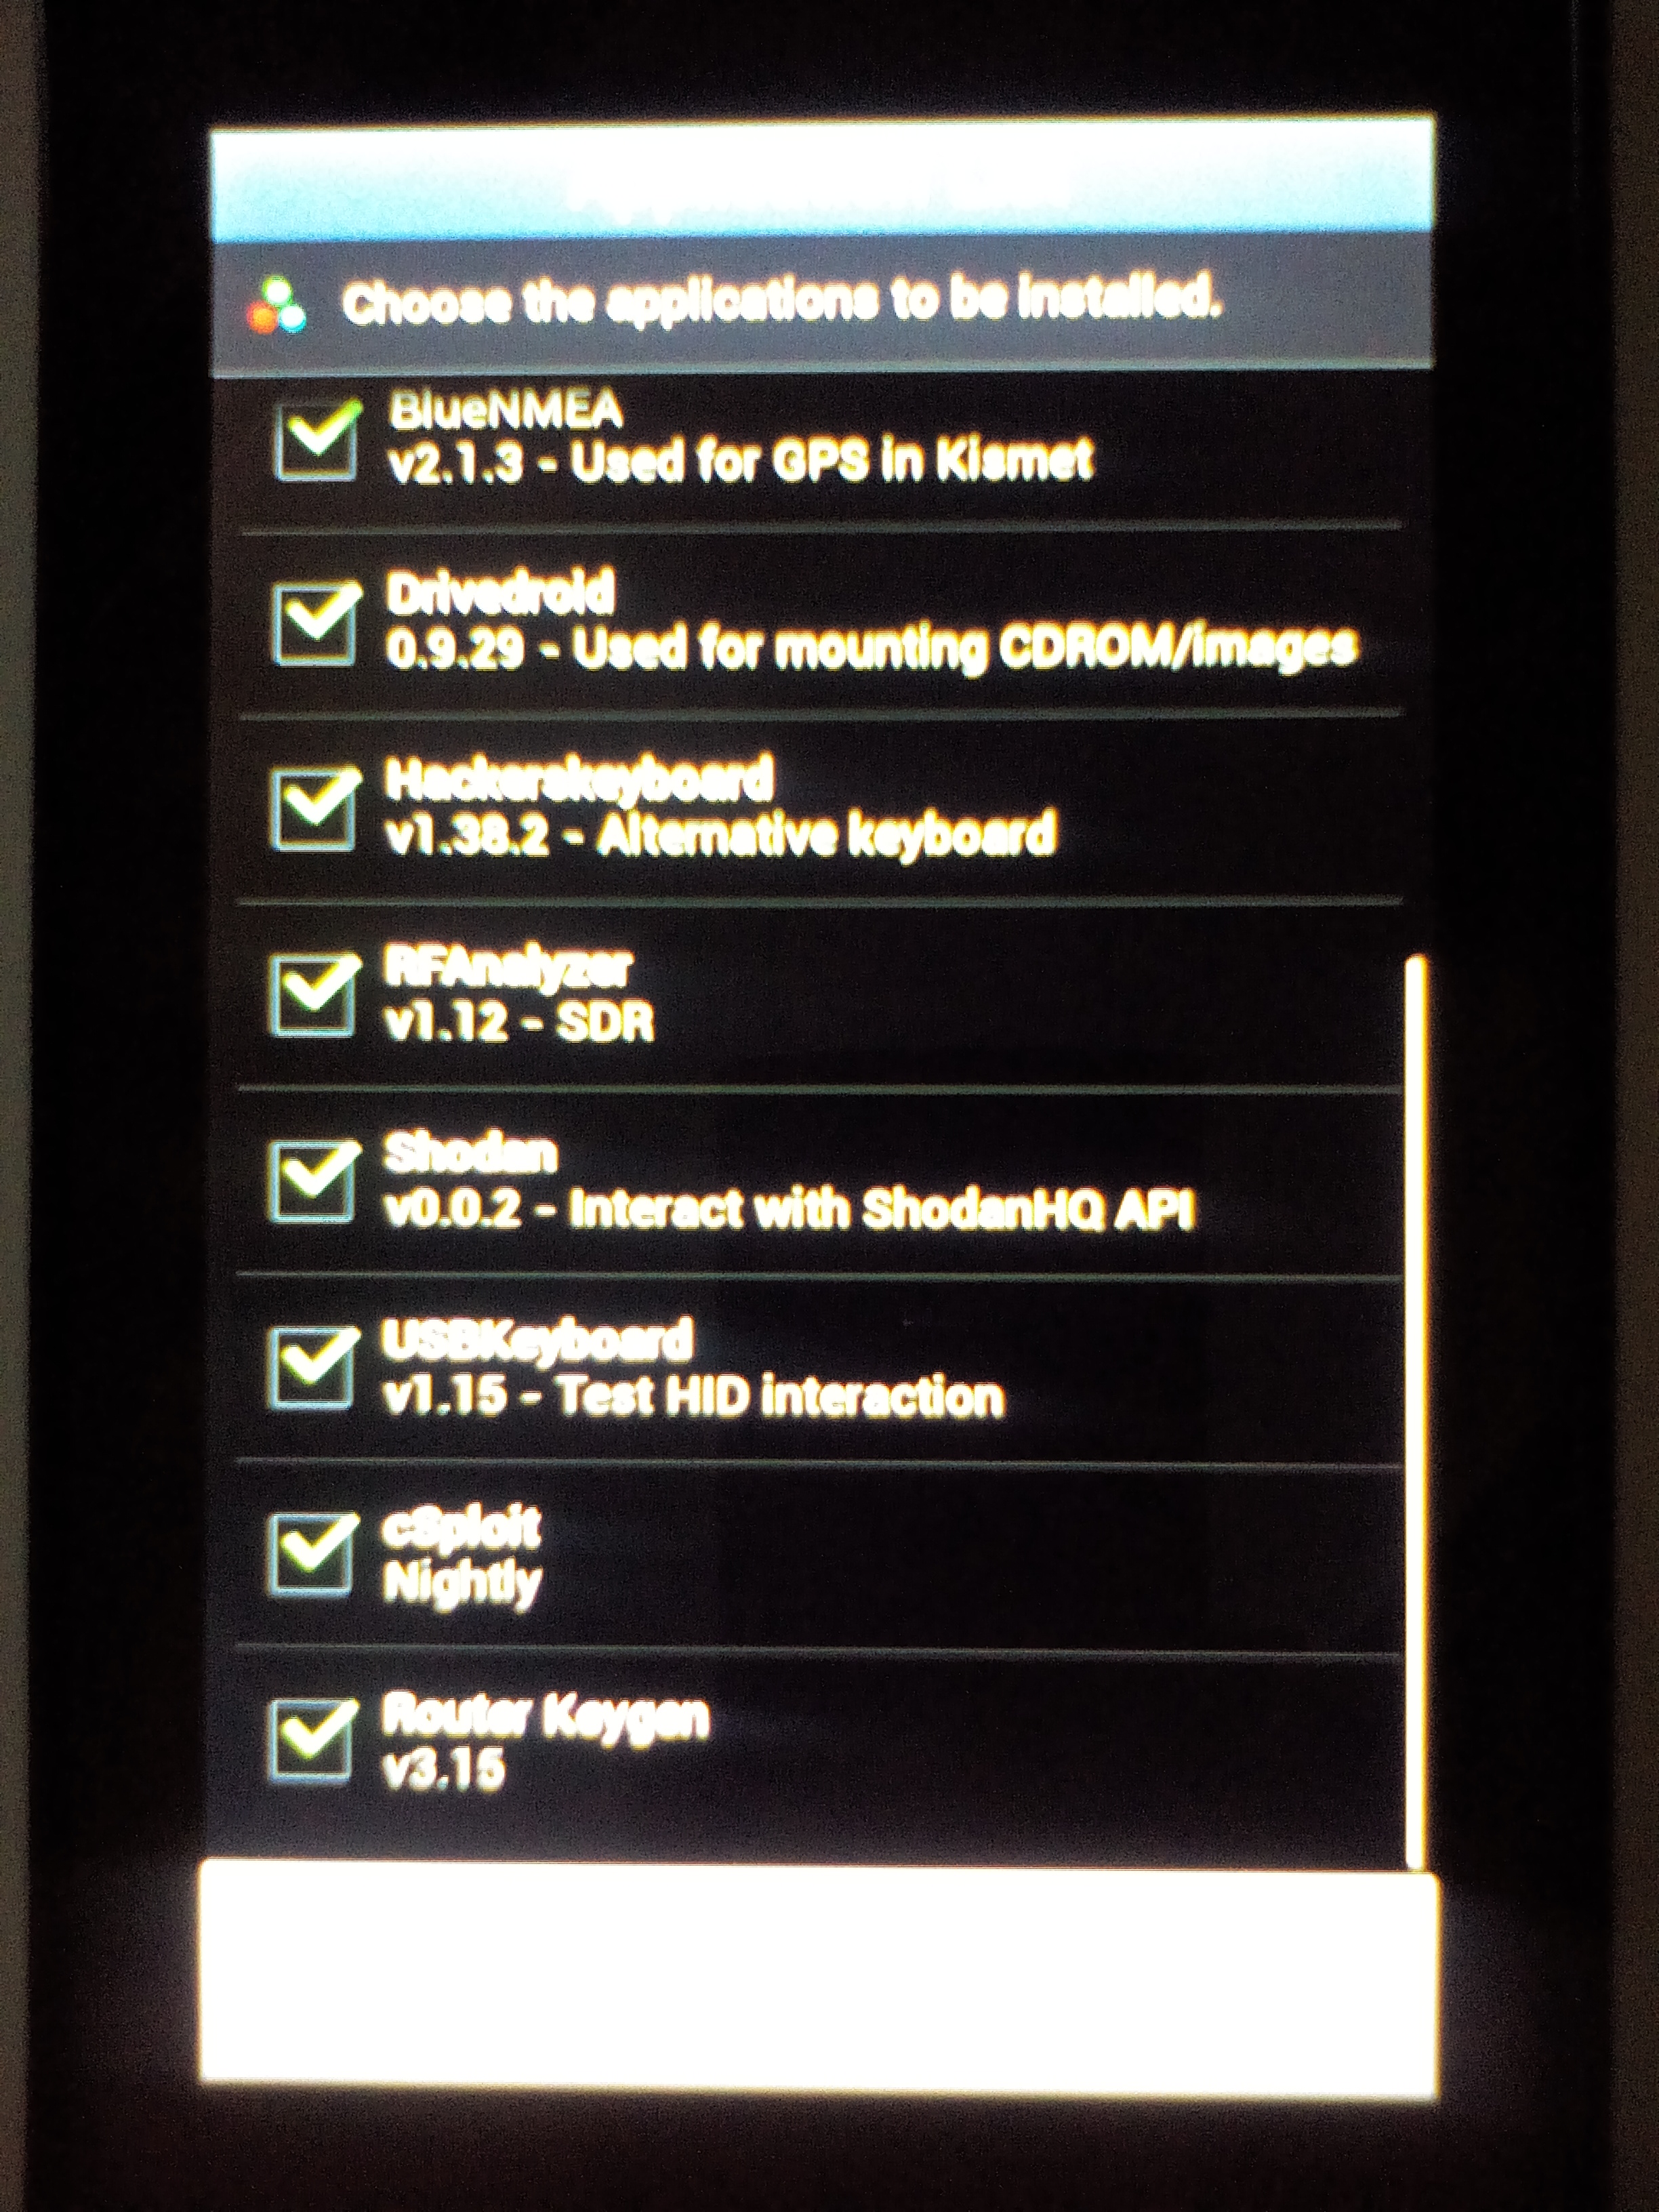
\includegraphics[scale=0.1]{./Image/img15}  \\
\caption{Anwendungen 2}
\end{center}
\end{figure} 

Endlich die Installation starten. Die Figure 16 zeigt das. \\
\begin{figure}[H]
\begin{center} 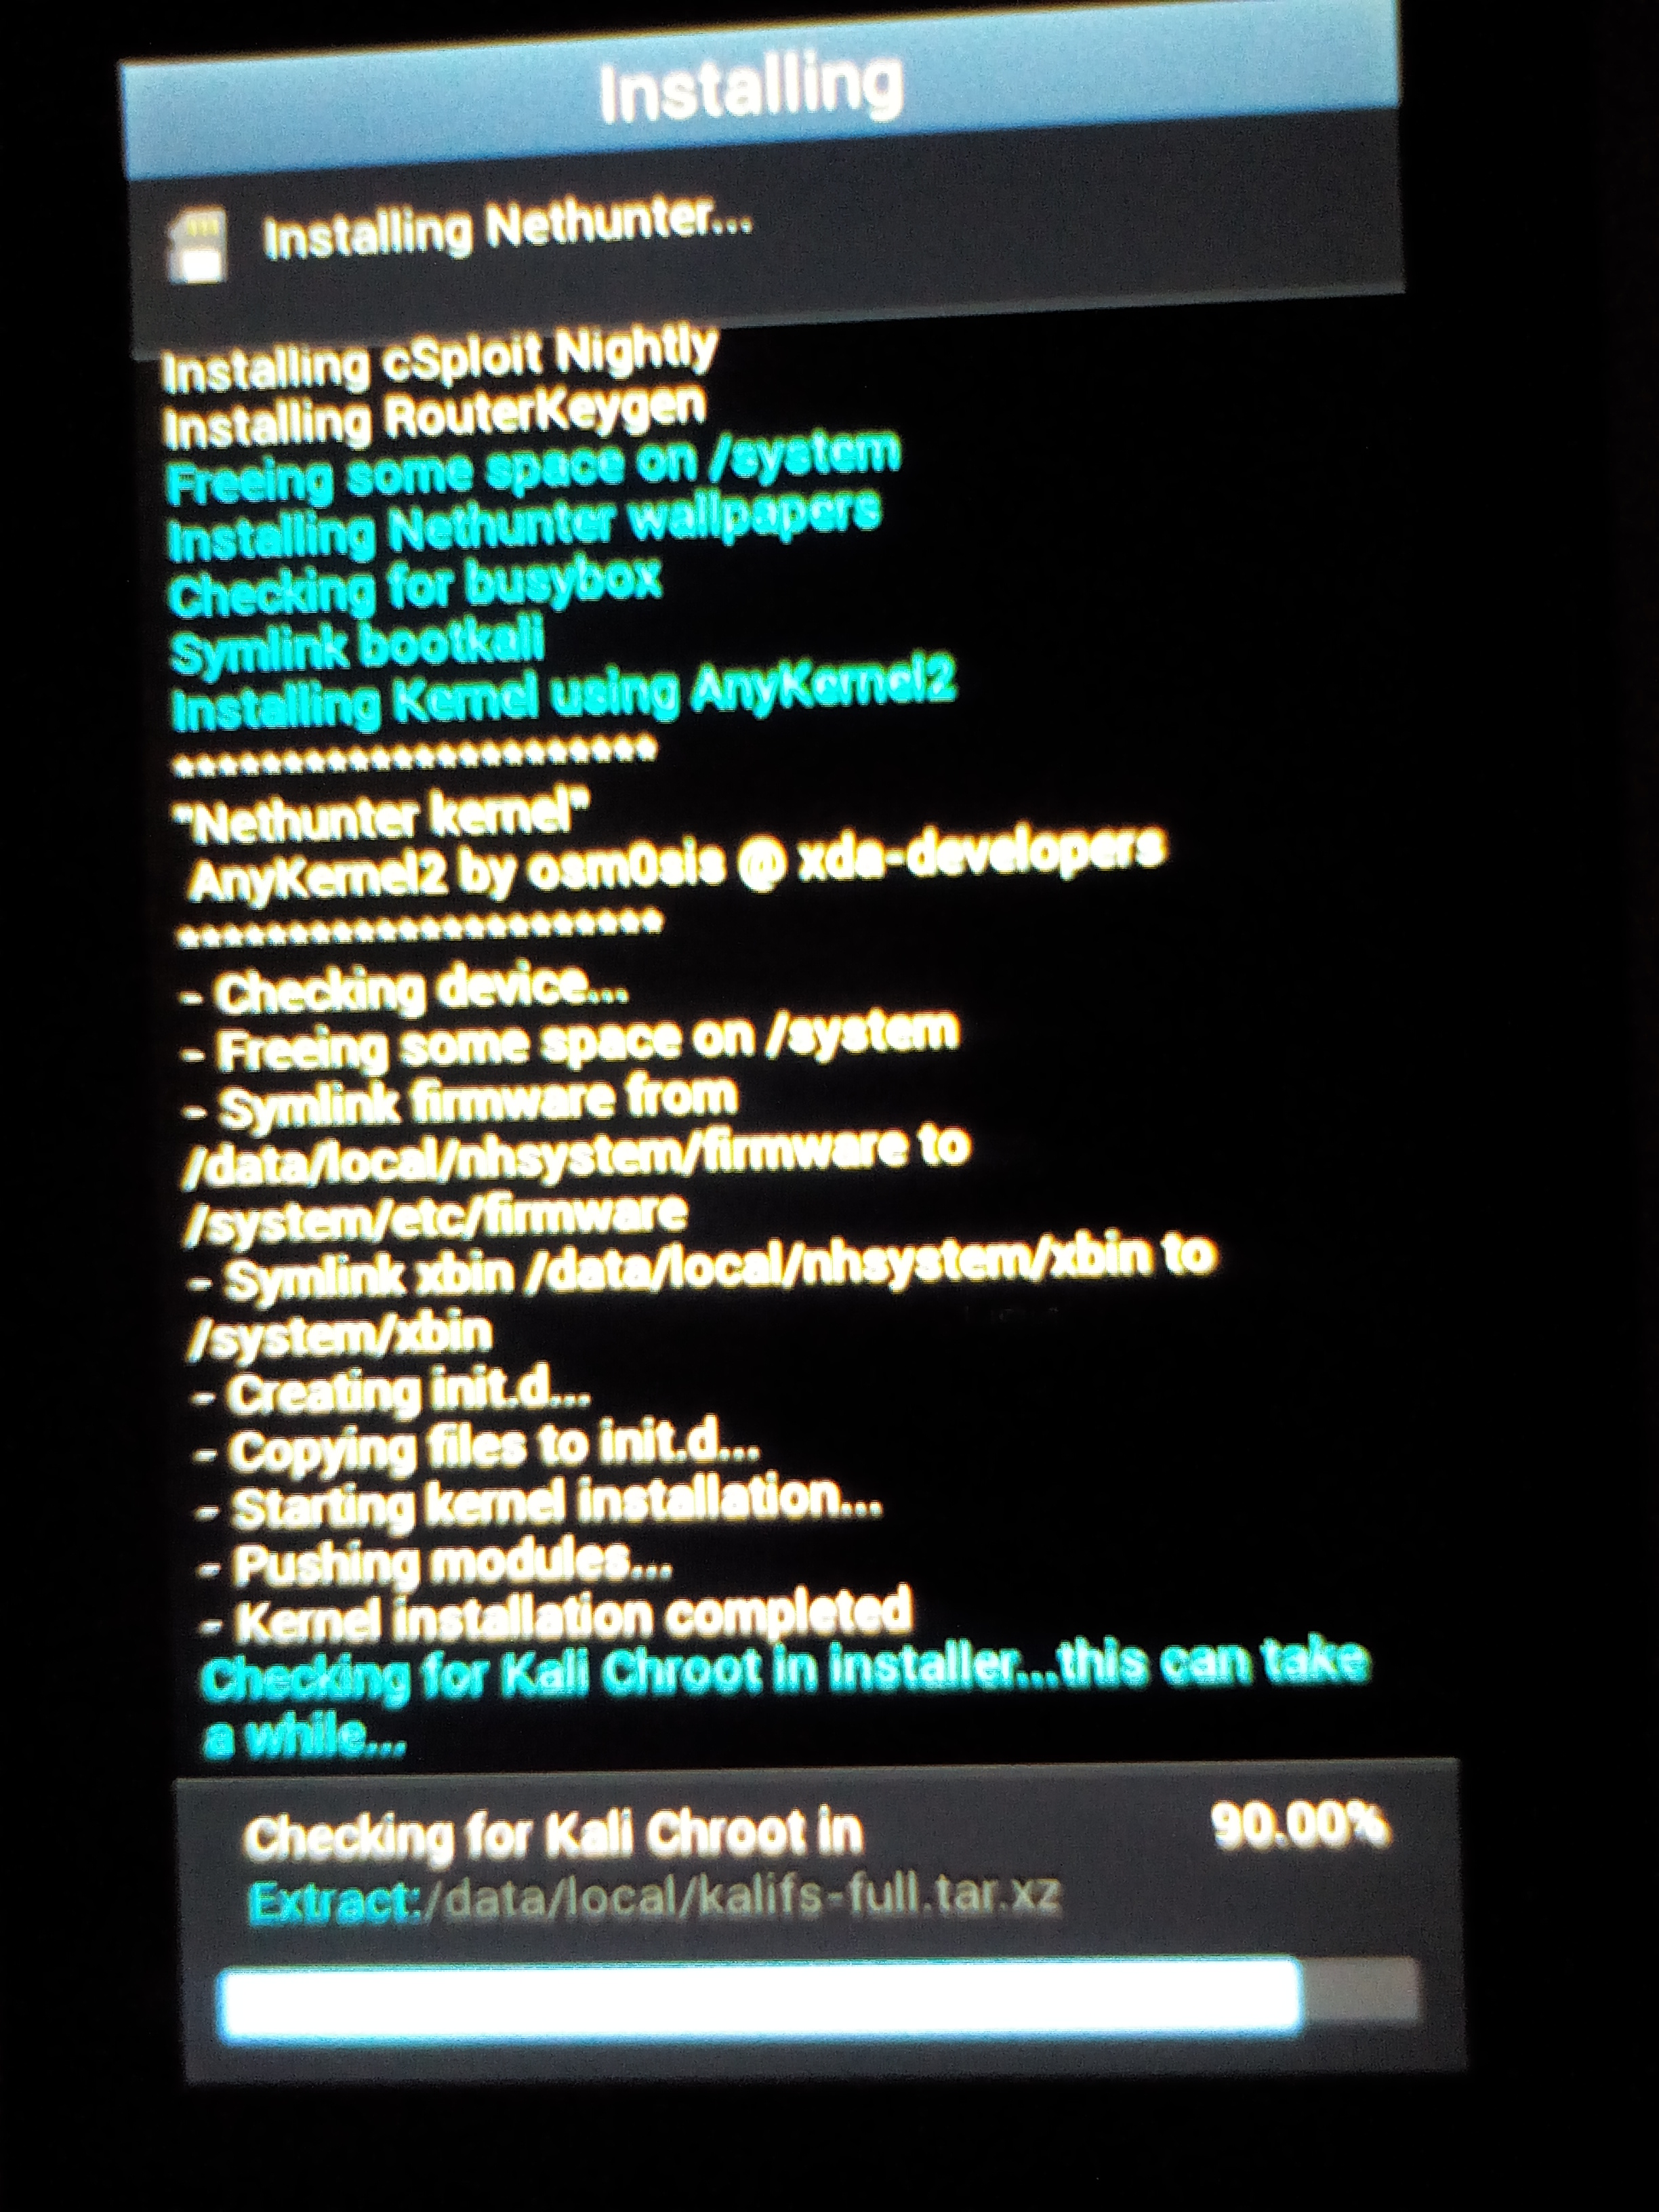
\includegraphics[scale=0.1]{./Image/img16}  \\
\caption{Anwendungen 2}
\end{center}
\end{figure} 

Literatur: Installing and und Running Kali Nethunter \footnote{
Literatur: http://www.beartechnology.com/Blog/Post/2/Kali-NetHunter-3-0-Installed-on-Nexus-7-(2012)-5-1-1-Lollipop}


\end{document}